% Define document class. Important.
\documentclass[a4paper,twoside,openright]{memoir}

% simple command to insert our final language name. Use \langname wherever you write the language's name.
% \newcommand{\langname}{InvaderScript}
%\newcommand{\langname}{Yo Mama}
\newcommand{\langname}{Dagor}


% Margener
%\setlength{\evensidemargin}{1cm}
%\setlength{\oddsidemargin}{1cm}

% Set up encoding. Latin1 since UTF-8 is fuckably difficult to work with.
% \usepackage[latin1]{inputenc}
\usepackage[latin1,utf8,ansinew]{inputenc}

% Variable, neat, references.
\usepackage{varioref}

% Acronym package. Makes it easier to introduce acronyms.
\usepackage{acronym}
% Add acronyms defined in separate file.
\acrodef{dm}[DM]{Dungeon Master}
\acrodef{rpg}[RPG]{Role-Playing Game}
\acrodef{rpgs}[RPGs]{Role-Playing Games}
\acrodef{vtm}[VTM]{Vampire: The Masquerade}
\acrodef{regex}[Regex]{Regular expressions}
\acrodef{cfg}[CFG]{Context-Free Grammar}
\acrodef{cfgs}[CFGs]{Context-Free Grammars}
\acrodef{bnf}[BNF]{Backus-Naur Form}
\acrodef{ebnf}[EBNF]{Extended Backus-Naur Form}
\acrodef{dnd}[DnD]{Dungeons \& Dragons}
\acrodef{wod}[WoD]{World of Darkness}

\usepackage{latexsym}

%Premable for semantic
%\input{semantic_preamble}

% Load up bibliography.
\usepackage[numbers]{natbib}
% Bibliography style.
\bibliographystyle{plainnat}

% Algorithm support.
\usepackage{algorithmic}
\usepackage{algorithm}
\usepackage{lastpage}
% Make algorithms appear as procedures instead.
\floatname{algorithm}{Procedure}
\renewcommand{\algorithmicrequire}{\textbf{Input:}}
\renewcommand{\algorithmicensure}{\textbf{Output:}}

% Image frames.
\setlength{\fboxsep}{0pt}
\setlength{\fboxrule}{0.5pt}

% Also, images.
\usepackage{graphicx}

% PDF includes
\usepackage{pdfpages}

% Block comments
\usepackage{verbatim}

% Todo notes here and there.
\usepackage{todonotes}

% Forbedrede floats.
\usepackage{float}

% Special symbols availability.
\usepackage{amsmath}
\usepackage{amssymb}
\usepackage{amsthm}

% CODE %
\usepackage{listings}
\usepackage{color}
\definecolor{gray}{rgb}{0.4,0.4,0.4}
\definecolor{darkblue}{rgb}{0.0,0.0,0.6}
\definecolor{cyan}{rgb}{0.0,0.6,0.6}
\lstset{
  basicstyle=\ttfamily,
  columns=fullflexible,
  showstringspaces=false,
  commentstyle=\color{gray}\upshape,
  basicstyle=\small,
  numberstyle=\footnotesize,
  numbers=left,
  captionpos=b,
  stepnumber=1,
  numbersep=10pt,
  tabsize=2,
  breaklines=true,
}
% Define markup of XML
\lstdefinelanguage{XML}
{
  morestring=[b]",
  morestring=[s]{>}{<},
  morecomment=[s]{<?}{?>},
  identifierstyle=\color{darkblue},
  keywordstyle=\color{cyan},
  morekeywords={id, target, type, category, value, point, correct, rows, width, time}% list your attributes here
}
% Define markup of C#
\lstdefinelanguage{CSharp}[Visual]{C++}
{
	identifierstyle=\color{darkblue},
	commentstyle=\color{green!70!black}\itshape ,
	stringstyle=\color{gray},
	sensitive=true,
	morestring=[b]",
	morestring=[b]',
	morecomment=[l]//,
	morecomment=[n]{/*}{*/}
}
% Define markup of JavaScript - copied from:
% http://lenaherrmann.net/2010/05/20/javascript-syntax-highlighting-in-the-latex-listings-package
\lstdefinelanguage{JavaScript}{
  keywords={typeof, new, true, false, catch, function, return, null, catch, switch, var, if, in, while, do, else, case, break},
  keywordstyle=\color{blue}\bfseries,
  ndkeywords={class, export, boolean, throw, implements, import, this},
  ndkeywordstyle=\color{darkgray}\bfseries,
  identifierstyle=\color{black},
  sensitive=false,
  comment=[l]{//},
  morecomment=[s]{/*}{*/},
  commentstyle=\color{purple}\ttfamily,
  stringstyle=\color{red}\ttfamily,
  morestring=[b]',
  morestring=[b]"
}

% External file with definitions of languages.
\definecolor{dkgreen}{rgb}{0,0.6,0}
\definecolor{gray}{rgb}{0.5,0.5,0.5}
\definecolor{mauve}{rgb}{0.58,0,0.82}
\definecolor{orange}{rgb}{1,0.5,0}

\lstdefinestyle{ourstyle}
{
	keywordstyle=\color{blue},          % keyword style
	commentstyle=\color{dkgreen},       % comment style
	stringstyle=\color{mauve},         % string literal style
}

\lstdefinelanguage{ourlang}
{
	keywords = {[1]Character,Ability,Effect,Item,Attribute,Resource,Behaviour,Event,make,from,owner,this,self,enemy},
	morekeywords = {[2]attributes,resources,effects,abilities,items,events,targets,cost,behaviour,team,ally,target, mana_cost, positive, negative,name},
	sensitive = true,
	keywordstyle=\color{blue},          % keyword style
	keywordstyle={[2]\color{dkgreen}},
	commentstyle=\color{dkgreen},       % comment style
	stringstyle=\color{mauve},         % string literal style
}

\lstdefinelanguage{fflang}[]{ourlang}
{
	morekeywords = [20]{
		% Classes
		Warrior,WhiteMage,BlackMage,Monk,Ninja,Master,WhiteWizard,Knight,BlackWizard,
		% Attributes
		strength,intelligence,defense,magic,agility,
		%Resources
		health,mana,PhysicalDamage,Heal},
	keywordstyle={[20]\color{orange}}
}

% Neat-o referencer...o.
\usepackage{hyperref}
\usepackage{nameref}

% hack fra nettet.
% http://tex.stackexchange.com/questions/1230/reference-name-of-description-list-item-in-latex
\makeatletter
\let\orgdescriptionlabel\descriptionlabel
\renewcommand*{\descriptionlabel}[1]{%
  \let\orglabel\label
  \let\label\@gobble
  \phantomsection
  \edef\@currentlabel{#1}%
  %\edef\@currentlabelname{#1}%
%  \let\label\orglabel
  \orgdescriptionlabel{#1}%
}
\makeatother
% Rettehak. Meget lettere end \checkmark
\newcommand{\yes}{\checkmark}

% Let's put in a lot of niceness in the display, yeh?

\usepackage{color,calc,graphicx,soul,fourier}
\definecolor{nicered}{rgb}{.647,.129,.149}
\makeatletter
\newlength\dlf@normtxtw
\setlength\dlf@normtxtw{\textwidth}
\def\myhelvetfont{\def\sfdefault{mdput}}
\newsavebox{\feline@chapter}
\newcommand\feline@chapter@marker[1][4cm]{%
\sbox\feline@chapter{%
\resizebox{!}{#1}{\fboxsep=1pt%
\colorbox{nicered}{\color{white}\bfseries\sffamily\thechapter}%
}}%
\rotatebox{90}{%
\resizebox{%
\heightof{\usebox{\feline@chapter}}+\depthof{\usebox{\feline@chapter}}}%
{!}{\scshape\so\@chapapp}}\quad%
\raisebox{\depthof{\usebox{\feline@chapter}}}{\usebox{\feline@chapter}}%
}
\newcommand\feline@chm[1][4cm]{%
\sbox\feline@chapter{\feline@chapter@marker[#1]}%
\makebox[0pt][l]{% aka \rlap
\makebox[1cm][r]{\usebox\feline@chapter}%
}}
\makechapterstyle{daleif1}{
\renewcommand\chapnamefont{\normalfont\Large\scshape\raggedleft\so}
\renewcommand\chaptitlefont{\normalfont\huge\bfseries\scshape\color{nicered}}
\renewcommand\chapternamenum{}
\renewcommand\printchaptername{}
\renewcommand\printchapternum{\null\hfill\feline@chm[2.5cm]\par}
\renewcommand\afterchapternum{\par\vskip\midchapskip}
\renewcommand\printchaptertitle[1]{\chaptitlefont\raggedleft ##1\par}
\setsecindent{2pt}
\setsecheadstyle{\normalfont\Large\bfseries\scshape\color{nicered}}
\setsubsecindent{2pt}
\setsubsecheadstyle{\normalfont\large\bfseries\scshape\color{nicered}}
\setsubsubsecindent{2pt}
\setsubsubsecheadstyle{\normalfont\normalsize\bfseries\scshape\color{nicered}}
}
\makeatother
\chapterstyle{daleif1}


%\usepackage{fancyhdr} % Get some niceness into our headers.
%\pagenumbering{arabic} % Ensure page numbering in our desired form.
%\pagestyle{fancy}
% Page design from fancyhdr.
%\fancyhead{}
%\fancyfoot{}
%\fancyhead[RO,LE]{\leftmark\\\rightmark}
%\fancyfoot[C]{\thepage}
%\setlength{\headheight}{23pt}
% Rewrite header and footer commands.
%\renewcommand{\headrulewidth}{1.0pt}
%\renewcommand{\footrulewidth}{1.0pt}

% Create a new command, HRule, to insert some nice horisontal rules on the title page.
\newcommand{\HRule}{\rule{\linewidth}{0.3mm}}

% New command for two figures, side by side.
\newcommand{\twofigs}[6]
{
	\begin{figure}[H]
		\begin{minipage}[b]{0.5\columnwidth}
		\centering\fbox{\includegraphics[width=0.8\columnwidth]{img/#1}}\caption{#2\label{#3}}
		\end{minipage}
		\hspace{0.5cm}
		\begin{minipage}[b]{0.5\columnwidth}
		\centering\fbox{\includegraphics[width=0.8\columnwidth]{img/#4}}\caption{#5\label{#6}}
		\end{minipage}	\end{figure}
}

% Sørg for at paragrafplads ikke spildes.
\raggedbottom

\begin{document}

\thispagestyle{empty}
{\begingroup
\raggedleft
\vspace*{\baselineskip}
{\color{nicered}\HUGE\bfseries \langname{} \\ \Huge and Batteru Enjin}\\[\baselineskip]
{\color{nicered}\large\bfseries A declarative language for describing RPG battles}\\[0.1\textheight]
{\color{nicered}\Large Project group SW406F12}\par
\vfill
{\Large \sffamily Aalborg University, Department of Computer Science\\
\hfill SW4, spring semester 2012}
\vspace*{\baselineskip}
\endgroup}


\begin{comment}
\begin{center}
	%\includegraphics[width=15cm]{forside.png}\\~\\
	\hrulefill\newline
	\\
	\begin{LARGE}	
	\textbf{\langname{} and Batteru Enjin}
	\end{LARGE}
	\\
	\begin{large} 
	\textbf{A declarative language for describing RPG battles.}
	\end{large}\\
	\hrulefill\newline
	%\hrule
	\\~\\
	Aalborg University, Fourth semester at Department of Computer Science \\
	SW4, spring semester 2012	\\
	Project group SW406F12\\
\end{center}
\end{comment}
\newpage
\thispagestyle{empty}
\mbox{}
\clearpage

% Dette er LaTeX-versionen af titelbladet for tek-nat-basis-rapporter 2004 efter�r
% Filen kr�ver:
% Universitetets logo:  aau-logo.png (for LaTeX) eller aau-logo.ps (for LaTeX)
% Synopsis: En fil ved navn synopsis.tex

% Udarbejdet af: Hans H�ttel (hans@cs.auc.dk) 21. maj 2003
% Rettet af Morten Christophersen (mortench@tnb.aau.dk) 30. nov 2004(�ndret til nyt design 2004 efter�r)

%\documentclass[11pt]{article}
%\ifx\pdfoutput\undefined 
%\usepackage[dvips]{graphicx}
%\else
%\usepackage[pdftex]{graphicx} 
%\usepackage{type1cm} \fi
%    \usepackage[ansinew]{inputenc}
%    \usepackage{a4}

%\begin{document} 
\phantomsection
\pdfbookmark[0]{Titelblad}{titelblad}
\thispagestyle{empty}
%\begin{titlepage}
\begin{nopagebreak}
{\samepage 
\begin{tabular}{r}
\parbox{\textwidth}{\begin{tabular}{l}
{ \raisebox{15mm} {
\includegraphics[height=1.2cm]{img/aau-logo.pdf}} }\\
{\textbf{Student report}}
\end{tabular}
\hfill \parbox{8cm}{\begin{tabular}{l} %4.90
{\small \textbf{Department of Computer Science}}\\
{\small Selma Lagerl�fs Vej 300} \\
{\small DK-9220 Aalborg �st} \\
{\small Telephone +45 9940 9940} \\
{\small Telefax +45 9940 9798} \\
{\small http://cs.aau.dk} 
\end{tabular}}}
\end{tabular}


\begin{tabular}{cc}
\parbox{7cm}{
\begin{description}

\item { Title:} 

A declarative language to describe battles in RPG scenarios. \\
  
\item { Theme:} 

Design, Definition and Implementation of Programming Languages

\end{description}

\parbox{8cm}{

\begin{description}
\item { Project period:}\\
   4th semester 2012 SW
  \hspace{4cm}
\item { Project group:}\\
  SW406F12
  \hspace{4cm}
\item { Group members:}\\
Birgir M. Eliasson \\
Johannes L. Borresen\\
Ren� K. H. Andersen\\
Barbara A. Flindt\\
Jeppe B. Tarp\\
  \hspace{2cm}
\item { Supervisor:}\\
Danny B�gsted Poulsen\\
  
\end{description}
}
\begin{description}
\item { Circulation: 8 }
\item { Number of pages: \pageref{LastPage} } 
\item { Number of Appendices: 4 } 
\item { Finished: 19-12-2011 }
\end{description}
\vfill } &
\parbox{7cm}{
  \vspace{.15cm}
  \hfill 
  \begin{tabular}{l}
  { Synopsis:}\bigskip \\
  \fbox{
    \parbox{8.2cm}{\bigskip
     {\vfill{\small This project is based on an Android system developed by four sixth semester groups in the spring semester of 2011 - it was called GIRAF. Based on the vision of a PC-based tool for administering GIRAF application and in cooperation with Birken (a kindergarten for children suffering from autism), this project expands the original concept into one a web-based framework for administration of GIRAF and tools focused on the communication between the various interest groups in play. Due to time constraints, only a part of the system was implemented, concentrating on the development of a digital contact book, to replace the physical books currently in use at Birken.

% This project is based on an Android system made in a bachelor multiproject in 2011. The developed system was called GIRAF. The initializing problem from the original project proposal, was to make a PC tool, used for administration of the applications developed for the GIRAF system. During the project the group has been cooperating with Birken, which is a institution for autistic children. After the first meeting with the representative Kristine Niss-Henriksen, the focus of the project was changed from making an administration tool, to making a digital version of a contact book; like the one used by Birken to communicate between the institution and the parents.

The report specifically describes the development of the central notion of a GIRAF administration system, singling out the contact book. The final system is implemented using web technologies (HTML, CSS, PHP, JS) in a Model-View-Controller architecture. Finally, the system's functionality and usability is lightly tested.

%This report describes the development of GIRAF administration system with main focus on the contact book. This report includes the usage of models, prototypes, the client-server architecture, and the implementation of the model-view-controller design. Furthermore to evaluate the system both unit testing and usability testing were used.
     \bigskip}}
     }}
   \end{tabular}}
\end{tabular}}
\\ \\\\\\
\noindent{\footnotesize{\textit{ This report is produced by students at AAU. The content of the report is freely accessible,
but publication (with source) may only be made with the authors consent}}}
\end{nopagebreak}
%\end{titlepage}
%\end{document}

\newpage
\thispagestyle{empty}
\mbox{}

\chapter*{Preface}
The following report has been made as a part of the SW3 project for the second-year students of software engineering at Aalborg University. The report is based upon the project proposals given to the students at the beginning of the semester and written in parallel with the lectures \emph{Algorithms and Data Structures}, \emph{Systems Development and Design}, \emph{Implementation and Evaluation of User Interfaces}. Source material can be found in the last part of the report.

The group would like to thank the Kindergarten Birken and their kindergarten teacher Kristine Niss-Henriksen for her participation in this project. This report and product is an expansion of the multi-project from spring 2011 made by the groups: s601a, s601b, s601c and s601e, and we want to thank these groups for the pre-work. Finally, we want to thank our supervisor Ulrik Nyman, for his continued envolvment and support during this process.

\phantom{Luft}

\phantom{Luft}

\begin{table}[H]
	\centering
		\begin{tabular}{c c c}
			\underline{\phantom{JAERJAERJAERJAER}} & \underline{\phantom{JAERJAERJAERJAER}} & \underline{\phantom{JAERJAERJAERJAER}} \\
			Birgir M. Eliasson			& Christoffer Kjeldgaard       	& Johannes L. Borresen 			\\
			&&\\
			&&\\\\\\
			\multicolumn{3}{c}{\underline{\phantom{JAERJAERJAERJAER}}} \\
			\multicolumn{3}{c}{Barbara} 			\\
			&&\\
			&&\\\\\\
			\underline{\phantom{JAERJAERJAERJAER}} & \underline{\phantom{JAERJAERJAERJAER}} & \underline{\phantom{JAERJAERJAERJAER}} \\
			Jeppe K�lling Tarp			& Ren� K. H. Andersen 					& Toke N. Olsen				\\									
		\end{tabular}
\end{table}


\newpage
\thispagestyle{empty}
\mbox{}

%\newpage
%\thispagestyle{empty}
%\mbox{}

%\newpage
%\thispagestyle{empty}
%\mbox{}
%\fancyhead{}
%\fancyfoot{}
%\fancyhead[RO,LE]{\leftmark\\\rightmark}
%\fancyfoot[C]{\thepage}
%\setlength{\headheight}{23pt}

% Fjern headeren for indholdsfortegnelsen.
%\fancyhead{}
%\fancyfoot{}
%\fancyhead[RO,LE]{\leftmark}
%\fancyfoot[C]{\thepage}
%\setlength{\headheight}{23pt}% Indholdsfortegnelser etc.
% Dybde for visning af niveauer.
% Dybde af niveaut�lling generelt.
\setcounter{secnumdepth}{3}
\setcounter{tocdepth}{1}

\tableofcontents

% 1. Intro
\chapter{Introduction}


To communicate with a computer, one is required to 'speak' the same language as the computer. A computer's language is pre-defined by the producer of the computer, and generally referred to as \emph{machine code} or \emph{machine instructions}.\\
Today's software developers make use of various programming languages and each language deals with an area of functionality. These languages have to be translated for the computer and this is done with tools called compilers.\\
When developing, the choice of programming language can be vital to the project's success and functionality.\\\\
In this report, a description of the development-process of a new language is laid out.

\section{\langname{}}
In this project it is wanted to address the interest for a role-playing based language. The purpose of the language is to define characters, skills, attributes, effects etc, commonly found in \ac{rpgs}.

To do this a language is constructed, which should catch the intuitive and simple characteristics of character sheets. Character sheets can be thought of as information containers for various \ac{rpgs}. They keep track of the character's skill- and health-state as well as inventory (for reference see appendix \vref{charsheet}).

\section{Role-playing}
\ac{rpgs} have been commercially available since the 1970's and exist in various forms. \ac{rpgs} can be described as interactive storytelling, meaning that the players take part in ''writing'' the adventure being played. When actions are unrestricted and players are free to do as they please the adventure becomes more than a story, evolving into an interactive activity between the players and the storyteller.
There are currently three types available; \emph{Computer-}, \emph{\ac{pnp}-} and \emph{Live Action \ac{rpgs}}, the first two being a focus in this project.

In \ac{rpgs}, players take on the roles of fictitious characters, most often created by the players themselves.

When playing \emph{\ac{pnp}- \ac{rpgs}}, a core rulebook is used, to solve conflicts, get inspiration for adventures, character creation, reference and more. In \emph{Computer- \ac{rpgs}}, the rulebook is replaced with static rules implemented in the game world, however developers often provide useful information (much like rulebooks) for the players in the form of a guide or a codex.
Characters are defined by their abilities and attributes, meaning that each ability is assigned a number that represents how 'good' the character is using a given ability. This is also the case with attributes and certain 'traits' (e.g superpowers and disciplines). An attribute is value on a scale of some minimum number to some maximum, where each value indicates how much better or worse a character is compared to other beings in the game world. Take for example the attributes strength and charisma. Strength tells you how strong a character is, often used to measure how much they can lift and how hard they can hit. Charisma is a character's social skill level, used to measure how well they can handle social situations. Most games break as much as possible down to numbers; appearance, intellect, luck and more.
This should in a way contribute to the level of realism in events and outcomes while playing.

The first modern \emph{\ac{pnp} \ac{rpg}} to be released commercially is the game \emph{\ac{dnd}}, which was first published in 1974.\cite{wikidnd}
\emph{\ac{dnd}} can therefore be thought of as the pioneer of role-playing games.

\subsection{Character creation}

How a character is created varies from system to system. Common for most is that the characters all have statistics (stats) describing them.
Stats are the term used for all numerical values in the character description. They can indicate a certain status amongst peers (e.g on a scale of 0 - 10), serve as a counter for how often a certain ability or item can be used, tell a character's level of skill and/or trait (such as Strength) and last but not least they keep track of the character's resources (such as \ac{hp}).
\ac{hp} is a measure for how much damage a character can take before dying. Strength can be used to calculate how much damage a character can do to others. Depending on what stat is in question, it can be decided by rolling dice, be computed from other stats, assigned specifically by the player or based on the player's choice of race.

\subsection{Pen \& Paper}
\todo{More details about GM}
When playing \emph{\ac{pnp}} the players generally use various dice (see figure \ref{dice}) to determine an outcome of an activity, for example an attack, where the outcome determines if the attack is successful and thereafter how much damage is inflicted. To help keep track of a character's attributes and other information, a character sheet is used.

In \ac{pnp} games the participants are: A \ac{gm}, who is responsible for control of non-player characters, environment, the setting of the adventure and has the final say in conflicts. The players control their individual characters, around which the adventure revolves.

A game scenario can be described as following: The \ac{gm} prepares an adventure for the players and lays down additional rules if needed. Participants are seated around a table with their character sheets and a number of dice. Each player has created a character to use in the given adventure. The \ac{gm} describes the setting and series of events, playing all non-player characters. The players roleplay their characters and determine their actions by themselves. When an action is required from a specific player, they can determine the outcome of the action by rolling a specific set of dice.
\begin{figure}[!h]
\centering
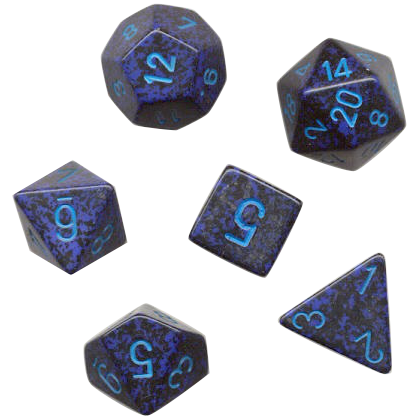
\includegraphics[scale=0.35]{img/rpgdice.png}
\caption{Dice for role-playing purposes}
%\cite{rpgdice}
\label{dice}
\end{figure}

\subsection{Digitised}
In \emph{Computer \ac{rpgs}} the outcome of an activity is determined by measures implemented by the developers. This can be an imitation of a dice roll (variation) or a static calculation (pre-calculated).
To keep track of character information, a digitised character sheet is often accessible, where the player can customise their character to some degree.\\
In computer \ac{rpgs} the player will often be given a set of possible actions to choose from, and it is up to the player to determine which one suits the situation best. The opponents are pre-programmed to react in a certain way to various events, such as low \ac{hp}.

\pagebreak

%source: (wikidnd) http://en.wikipedia.org/wiki/History_of_role-playing_games

\section{Initiating problem}
Combat scenarios are an integral part of many role-playing systems and games, but there are no languages that allow roleplayers with no programming experience to write and execute combat situations on their computers. 

This leads to the following initial problem:

\emph{"There is currently no language specialised in describing turn-based battles in computer role-playing games}
\begin{comment}
\emph{"While the game-development industry is continuously growing and role-playing games are so popular, why isn't there an RPG-based programming language available?"}
\end{comment}

%TODO Needs refurbishing, comments for fixes below....

%
%Why is it necessary to program imperative to develop games?
%Tala um low-level (c++ game engine stuff)
%Tala um high-level (scripting.. .sem er -�a� sem vi� erum a� gera)

%In this project, we want to design and construct our own programming language along with the tools to translate and make use of the designed language.
%This presents us with following tasks:
%\begin{itemize}
%	\item Designing a language
%	\item Designing a fitting grammar for the language
%	\item Designing and implementing an engine to showcase the capabilites of the language
%	\item Designing and implementing a compiler to translate the language for our engine
%\end{itemize}

%This brings us to an initial problem statement:\\
%\emph{\textbf{How do we efficiently design and implement a readible and writable language, capable of simplifying entity creation for a Role-playing game.}}

%source: http://www.theesa.com/facts/pdfs/ESA_EF_2011.pdf (ESA_EF_2001.pdf) statistics about games sold 2011

% 2. Analysis (RPG games and target audience)
\chapter{Analysis}

%Some analysis to come...
\section{Analysis of Role-playing systems}
Our target-group consists of people experienced in role-playing, both digital games and \emph{Pen \& Paper} games. Question sheets were created and sent out to a part of our target group, where questions regarding role-playing experience (number of known systems, years played, etc) and programming experience were answered. This helped us with designing our language to the needs of the target group.
After analysing the question sheets\vref{qsheets} we decided to take a closer look at three systems, described in the next section. The reason for this, is to find common characteristics and try to adjust our language to the basic needs of these popular role-playing games.

\subsection*{Role-playing games}

The World Of Darkness (WoD) is a supernatural horror role-playing game, which incorporates a system called \emph{Storytelling System} developed by \emph{White Wolf Inc}. It's world consists of mythical creatures like vampires, werewolves and ghosts. The system is unique in the way it handles character health and damage, which is categorising received damage and assigning a symbol to each type, making it easy to keep track of changes. The outcome of events is decided with one or more 10-sided dices.\cite{wod}

Dungeons \& Dragons (DnD) is a fantasy role-playing game, which incorporates a system called \emph{d20 System} developed by \emph{Wizards of the Coast}.
It's world consists of mythical creatures like elves, dwarves, dragons and other supernatural beings. The fact that the system is the first to be published commercially makes it an interesting reference. The outcome of events is decided with a dice pool containing 4-sided up to 20-sided dices, the 20-sided ones are used to roll for success (use abilities).\cite{dnd}

Cyberpunk 2020 (Cyberpunk) is a role-playing game with a postmodern science-fiction setting, which incorporates a system called \emph{Interlock System} developed by \emph{R. Talsorian Games}. It's world consists mostly of humans, cyborgs and robots.
The \emph{Interlock System} is skill-based instead of the traditional level-based system. Meaning that players get awarded points to spend on their skill sets instead of experience points. The outcome of events is decided with a similar dice pool to 'DnD, but using 10-sided dices to roll for success.\cite{cyberpunk}

\subsection*{Common characteristics}
\label{baseclasses}
The systems have some basic requirements to provide optimal playing experience, such as:
Character classes, attributes, effects, abilities, resources, modifiers and variation (dice rolls). These core entities represent their respective real-life concepts and the dice rolls introduce 'luck' to the mix.
Each of these systems have their 'dice pool' and their rules which define what types of dices and how many are involved in a given task.
The systems' dice size and quantity differ, but are derived from the same concept: \textit{''To decide the outcome of a given task, you must roll a dice of a specific size, add modifiers, calculate the result and compare to the task's difficulty. If your result is higher, you succeed''}\\

What these systems have in common, although implemented differently in each, is health points, damage and their calculations. This results in a different approach to our engine's damage calculations. While \ac{wod} and \emph{Cyberpunk} have some very convenient representations for \emph{pen \& paper} role-play, they are not suitable for our engine, reason being that health has various types, be it bashing, lethal or aggravated.
With this implementation the system captures some real-life forms of damage. An attack with a knife therefore does not have the same effect as with a hammer. Whereas in a health-resource based implementation, like in some video games, an attack does an amount of damage regardless of the type of attack. The amount is then subtracted from the health pool of the victim.
A character sheet from the game \ac{wod} is presented for reference on appendix \vref{charsheet}. As seen on the character sheet, a character is defined by their \emph{Attributes}, \emph{Skills} and \emph{Other Traits}. When playing a game, it is recommended to have the core rulebook as support, since calculations and various details about happenings is defined there.

\subsubsection*{Conclusion}
As a proof of concept, we choose the common characteristics of these systems for constructing the rulebook, common characteristics being the before mentioned \emph{requirements} of the systems.
By using Characters classes, attributes, effects, abilities, resources and modifiers, we can define a character in our language, like it was a character sheet. If done correctly, this should satisfy our target group.

\begin{comment}
\subsubsection*{''Final Fantasy'' \& engine specifics}
The Event system and fight simulation will be based on the first games of the video-game series \emph{Final Fantasy}, this is done to simplify the implementation. Final Fantasy is a fantasy role-playing game, released for the \emph{Nintendo Entertainment System} in 1987. The game was a success and has since then spawned a whole franchise named after the original title.
The Final Fantasy series have implemented various combat systems, turn-based and real-time.\cite{ffantasy}
Since our engine simulates battle and provides fairness through modifiers, we choose turn-based combat, where a battle is measured in turns.
For simplicity we also choose to restrict the number of contestants to two.
\end{comment}


%sources: WoD - The World of Darkness (ISBN: 1-58846-484-9) by White Wolf Publishing
%sources: Cyberpunk 2020: The Roleplaying Game of the Dark Future (ISBN: 0-937-279-13-7)
%sources: Dungeons & Dragons Player?s Handbook: Core Rulebook I, v. 3.5  (ISBN: 0-7869-2886-7)
%sources: Gameplay of Final Fantasy (http://en.wikipedia.org/wiki/Gameplay_of_Final_Fantasy)
\section{Language paradigms}
Within computer programming, a \emph{paradigm} is a model or framework for problem solving. \citeauthor{paradigms1992} describe it thus:

\begin{quote}
A programming paradigm is a collection of conceptual patterns that together mold the design process and ultimately determine a program's structure.
\end{quote}

The granularity with which paradigms are defined varies somewhat between sources. While \citeauthor{paradigms1992} keeps to the understanding that a paradigm is a larger philosophy of solving problems computationally, other sources maintain that a paradigm can be considered on the level of techniques (\citeauthor{paradigms1978} on divide and conquer \cite{paradigms1978}). Within the context of this report, we constrain ourselves to the more abstract form as presented by \citeauthor{paradigms1992} in order to better represent the higher levels of paradigms. The point of the discussion is to present an overview of the major paradigms, their main points of interest and perceived strengths/weaknesses of each. The discussion of paradigms is important, as choosing a proper paradigm (or set of paradigms) is key in considering how the target users should work with the designed language.

\citep{paradigms1992} put the paradigms into three categories: \emph{operational} (where programs are described as step-by-step procedures), \emph{demonstrational} (a higher-level abstraction where an example is shown and the compiler must derive a procedure from it) and \emph{definitional} (solution properties are described, but the method of solving it is not). The demonstrational paradigms lie beyond the scope of this project owing to its "code-by-example" approach, going close to (or within) the domain of graphical programming. It will not be further discussed.

\subsection{Operational versus Definitional}
To more easily narrow down the field of optimal paradigms, first consider the two overarching categories of the operational and the definitional paradigms.

In solving problems, the operational paradigms focus on specifying the solution method in sequencial steps. The granularity and focus of this approach is beneficial as solutions can be specified very precisely and the corresponding result sets are at the very least clear. However, it also demands a certain degree of familiarity with mathematical and algorithmic approaches to defining solutions, two disciplines not often found outside of programming. A necessary effect of this is the strict sequencing of steps, each one creating a new data state.

In contrast, the definitional paradigms focuses on constraining the solution set. As stated by \citep{paradigms1992}:

\begin{quote}
In definitional paradigms, a program is constructed by stating facts, rules, constraints, equations, transformations, or other properties about the solution value set.
\end{quote}

The programmer is no longer required to specify \emph{how} to reach a solution, only what a correct solution should look like. This can, in principle, alleviate some of the more complex aspects of programming tasks, making the language notably easier for beginners, hobby programmers or non-programmers. With from this assumption, we shift our attention only to the definitional paradigms.

\subsubsection*{Functional}
The functional paradigms focuses on the serial application of functions to reach a desired solution. The basic approach can be likened to mathematical function definitions. For example, the mathematical function

\[
f(x) =
\begin{cases} \frac{x+3}{12} & x \texttt{ mod } 3 = 0 \texttt{ and } x \geq 9
\\
\frac{x}{12} & x = 12
\\
(x * 4)^2 & \sqrt{x} = 3
\end{cases}
\]

Where the computation of the function is based on conditions related to the function argument. A similarly structured approach in a functional (pseudo) language could look like so (recall that $\sqrt[2]{x} = 3 \Leftrightarrow x = 3^2$):

\begin{lstlisting}
// The function f as defined equivalently above.
func f(X)
	:= (X+3)/12 if (X % 3 == 0 and x >= 9)
	:= x/12 if (X == 12)
	:= pow(x*4,2) if (x == pow(3,2))

// Function calculate power of a number.
func pow(I,P)
	:= I*pow(I-1,P) if P > 0
	:= I if P=0
\end{lstlisting}

There are several features of note in this approach. First of all, the deeply ingrained conditionals. A particular computation (in this case, a line of code) is performed only if certain conditions hold. Flow control (or line ordering) is a second feature (or lack of the same) to note. The functional paradigm can be applied in such a way so the order of conditions in a function are of no consequence. Indeed, this can be seen in the implementation of the $pow$ function. In an imperative recursive implementation of $pow$, the conditional check for $P==0$ must come before the recursive step as each line is evaluated downwards. This does not need to be the case for the functional approach. During evaluation, each line's conditions are checked. How and when branching is performed varies between implementations. Some short circuit (first match, if any), others with either most conditions met or most percentage of conditions met. The printed example assumes the latter. In all cases, a mechanism for defaults must be supplied as well. One approach is to use the last line if nothing holds. This would be considered an operational - imperative - approach, somewhat contrary to definitional dogma. Another would explicitly specify the default case.

The particular strength of the functional paradigms is the release from control flows and program states (note the lack of any intermediate or long-term variables) while attempting to adhere to mathematical principles for function definitions. It is left to the programmers of the compiler or interpreter to derive the proper execution order and result set. There remains, however, a need for the user of the language to understand fundamental discrete mathematics in order to properly apply the paradigm to a problem.

\subsubsection*{Transformational}
Transformational paradigms define a problem solution by a series of transformations. For example, the input $17$ might be transformed to $108$ through the transformations $17 \rightarrow 119 \rightarrow 108$ (using $17 * 7 = 119$ and $119 - 11 = 108$). A program is specified by a number of \emph{gourds} (conditions) and \emph{actions} (transformations) that define the possible transitions the input may go through. In this sense it has similarities with the functional paradigm. The difference, however, lies in how the transformations are applied. Where the functional paradigm leaves it to the programmer to specify which functions should be used, the transformational expects the system to identify which transformation to apply at any given point. In this manner, the system will transform the input until no guard will match it. At this point, the result is returned.

\subsubsection*{Logic}
The logic programming paradigm makes use of Horn clauses to describe predicates and the facts that must hold true for the predicate to do so as well. Horn clauses are beyond the scope of this report, but for context a brief example is in order. using notation of boolean algebra, a horn clause could be written as 

\[
(c_1, c_2, \cdots , c_n) \rightarrow f
\]

should be read as ''if the conditions $c_1$ to $c_n$ all hold true, then fact $f$ must also hold true''. A program written in the logic programming style is comprised solely of clauses like this. The programmer must define sufficient facts (and a goal to be reached), and the compiler must be able to deduce the correct resolution of facts to reach this goal. The set of possible combinations that must be tested to find the solution very quickly becomes so large that algorithms used for solving the problem must be heavily optimised, and even small changes to the ordering of facts can markedly affect the performance of the program. While several algorithms with acceptable running times have been designed, it still remains a challenge for the programmer not only to supply sufficient facts to deduce a solution, but also in a manner that is not counter-productive to the overall running time of the programmer. While the latter can be argued to be a staple of any programming paradigm, none would have as great an impact as in the logic programming paradigm.

\subsubsection*{Form-based}
Perhaps one of the simplest examples of the form-based paradigm in use is a spreadsheet application such as Microsoft Office or LibreOffice Spreadsheet. Computations are specified via equations, and can entirely avoid explicitly defining a control sequence by virtue of their interdependence. An equation must be computable independently of its result (that is, circular references are not allowed). Any formula $x = f(y_1, y_2, \cdots , y_n)$ therefore requires that all $y_i$ be computable independently from $x$.

This paradigm's strong point is the form in which programming is done. It is analogous to filling out regular forms (tax forms, applications - even character sheets) and should come naturally to many users - as a consequence, the roles of programmer and user become very close entwined.

\subsubsection*{Dataflow}
The dataflow paradigm regards input as a flowing stream of data, passed through nodes in a network that apply a formula to the data. The sequence is determined by the programmer as it is with the functional paradigm, but the dataflow philosophy is very well suited for parallel processing of data. Several streams of data may flow through nodes, and their paths may be independent before or after they pass the node. At those points, individual threads could handle each stream through other nodes until they converge. Conversely, each node could be handled by an individual thread, awakened whenever sufficient streams had entered the node for processing, and sent back to sleep when not needed.

\subsubsection*{Constraint programming}
This paradigm might best be described as the programmer's equivalent to an equation solver. The intention is for the programmer to sufficiently \emph{constrain} the solution's value set. This does not mean to simply write out formula for the system to evaluate given certain input, but to instruct the system as to how the formula remains valid. Consider an equation

\[
y = x^3 + 12c
\]

In the case of form-based, functional or dataflow paradigms, one would expect that $y$ could be computed once appropriate values $x$ and $c$ have been input. Constraint programming, however, should support finding any variable once enough of the other variables have bene passed. Consequently, the equation

\[
\sqrt[3]{y - 12c} = x
\]

is programmatically equivalent. The system must be able to derive these equations and computational possibilities on its own, without the programmer (assuming the programmer properly constrained the problem).
\pagebreak
\section{Syntax theori}
% ~Hornbjerg
Every language, whenever it is English, German, or some other language, have some specified gramma, used for making sentence in the languages. The gramma of the languages is specified by rules, which desripe how to use the gramma corretly.   \\
Every sourcecode of a program, written in some programming language also consist of some sentence. Specify how a correct sentence in programming languages i written, the programming language uses a set of rules called the \textit{syntax} of the language. The syntax of a programming language can be descriped i deffirent ways, but in this section, we focus at three ways:
\begin{itemize}
\item{\ac{cfg}}
\item{\ac{bnf}}
\item{\ac{ebnf}}
\end{itemize}

\subsection{\ac{cfg}}
\ac{cfg} was first descriped in the middel of the 1950s by Noam Chromsky. A \ac{cfg} is a colloction of substitutions rules. The rules consist of two kinds of symbols; \textit{nonterminals} also know as \textit{variable} and \textit{terminals}. Each rule in a \ac{cfg} is formed as a line, which constist determents how substitut one (ore more) \textit{variables} with an other vaiable or terminal. \\
An example of a \ac{cfg} is 

\begin{tabular}{l l l}
$A$ & $\rightarrow$ & $0A1$ \\
$A$ & $\rightarrow$ & $B$ \\
$B$ & $\rightarrow$ & $\#$ \\
\end{tabular}

In the gramma above the rules shows that $A$ can be substituted by either $0A1$ or $B$. \\
The \ac{cfg} above will be called $G$, and the language which can be generated by the \ac{cfg} $G$ is called a \textit{context-free language} and is written $L(G)$, which means $L$ is generated by $G$.

\subsection{\ac{bnf}}
In 1959 a new formal notation used to specify the syntax of at programming language was introduced by John Backus, and the notation was later modified by Peter Naur, and the notation was called \ac{bnf}. \\
\ac{bnf} is an other way of descriping syntax of a programming language. Like a \ac{cfg}, a \ac{bnf} is a collection of rules, which also uses \textit{terminals} and \textit{nonterminals}. An example of \ac{bnf} used to descripe a simple Java assignment statement is written as

\begin{tabular}{l l l}
$<\texttt{assign}>$ & $\rightarrow$ & $<\texttt{var}> \; = \; <\texttt{expression}>$ 
\end{tabular}

where $<\texttt{assign}>$ is an abstract reprecentation of an assignment statement, and the rule specifies that $<\texttt{assign}>$ is defined as an instance of the abstraction $<\texttt{var}>$ followed by the `=' symbol, and then followed by the abstraction $<\texttt{expression}>$.

\subsection{\ac{ebnf}}
\ac{ebnf} is an extended version of \ac{bnf}. The \ac{bnf} has though time bin extended i several ways, and even though all the extenssions is not exactly the same, the are all called \ac{ebnf}. The extensions only makes the notation more readable and writeably, they does not enhance the descriptive power of \ac{bnf}. \\
One of the things included in one of the extensions of the \ac{bnf}, denotes an optional part at the right-side of the ``$\rightarrow$'', which is delimeted by brackets. for an example, an \textbf{\texttt{if-else}} statement, in the programming language C. The statement can be descriped

\begin{tabular}{l l l}
$< \texttt{if\_stmt}>$ & $\rightarrow$ $ \textbf{\texttt{if}} \; ( < \texttt{expression} > ) \;  < \texttt{statement} > \; [ \textbf{\texttt{else}} \; < \texttt{statement} > ]$
\end{tabular}

With use of \ac{bnf} the statement would be desriped \\

\begin{tabular}{l l l}
$< \texttt{if\_stmt}>$ & $\rightarrow$ &  $\textbf{\texttt{if}}  \; ( < \texttt{expression} > ) \;  < \texttt{statement} >$ \\
 & $|$ & $ \textbf{\texttt{if}} \; ( < \texttt{expression} > ) \;  < \texttt{statement} > \; \textbf{\texttt{else}} \; < \texttt{statement} > $
\end{tabular}
\section{The internals of the compiler}

A compiler is divided into several different phases: First of all, there is the source program file which is the input to the compiler. The code is scanned by the aptly named scanner phase, converting the code into a stream of tokens. The tokens of the language are the smallest units that represent something meaningful. These are then grammatically analysed, or parsed, forming what is called an Abstract Syntax Tree (AST). A semantic analysis on the AST is performed, with the help of a symbol table, which is a table of all defined identifiers and the relevant information attached to them, such as declaration, type, scope and so on. Finally the target code is generated in the target language and ready for execution. The process will be elaborated to provide a little background knowledge of the compiler construction, as described in \cite{Fischer2010}.

Below is an illustration:

\begin{figure}[ht]
	\centering
		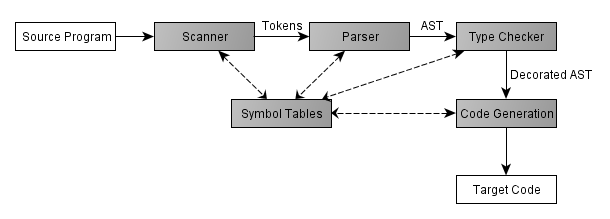
\includegraphics[scale = 0.5]{img/compiler.png}
	\caption{Compiler}
	\label{fig:compiler}
\end{figure}


\subsection{The Scanner}

The scanner is the part of the compiler responsible for transforming characters from the source program into a stream of tokens, i.e. the elementary symbols that define the language syntax, and the symbols that the parser can work with.
It is very important to have a formal definition of the tokens so that lexical rules are clearly stated and followed.
Tokens have two components: a type and a semantic value, the first indicating the token's membership in the terminal alphabet, the latter providing information about the token, if any is needed.
An example where the semantic value may not be needed is a terminal like "plus" in a simple calculator language. That terminal can only correspond to one token, namely the +. However for, say, a number it is important to have a semantic value to denote what number it is.
When the scanner tries to determine what kind of token is being scanned it will have a method that looks ahead, without removing the characters from the stream. Several algorithms for determining membership in the terminal alphabet can be employed, and often the scanner will also be instructed to skip certain parts of the code, like blanks and comment sections.
An example of the scanners token generation is shown below, with the lines
\begin{lstlisting}
i a 
a = 5
\end{lstlisting}

This generates 4 tokens: 
\begin{itemize}
\item A token of type "intdcl" (short for int declaration) with no need for a semantic value, as only the letter "i" corresponds to the type 
\item A token of type "id" with semantic value "a" 
\item A token of type "assign" with no need for a semantic value, as an assignment only corresponds to the "="
\item A token of type "inum" (short for integer numeral) with semantic value "5"
\end{itemize}

These tokens are then streamed to the parser. The process is illustrated below:
\begin{figure}[ht]
	\centering
		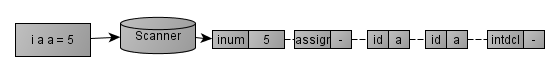
\includegraphics[scale = 0.6]{img/scanner.png}
	\caption{Scanner Phase}
	\label{fig:scanner}
\end{figure}


\subsection{The Abstract Syntax Tree}
The AST is a data structure generated by the Parser. It represents the structure of the source code. The root of the AST is the token representing the start variable in the grammar, e.g. "Program". The children of the root, and their children, are the variables or terminals that can be substituted for the parent. As an example, "Program" can be substituted with either "Decls" (declarations) or "Stmts" (statements) so these are the legal children of the root.

An AST of the tokens above is shown here:

\begin{figure}[ht]
	\centering
		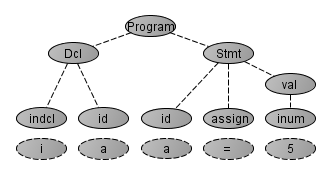
\includegraphics[scale = 0.7]{img/ast.png}
	\caption{Abstract Syntax Tree}
	\label{fig:ast}
\end{figure} 

\newpage
\subsection{The Parser}

The parser is the phase of the compiler that generates the AST. It checks whether the tokens generated by the scanner conform to the syntactical structure defined by the grammar of the language. 

There are several ways to handle the parser problem, i.e. the problem of creating the parse tree from the token stream. Some parsers create the tree from the root to the leaves, called top-down or LL parsing, others create the tree from the leaves up, called bottom-up or LR parsing. 

Top-down parsing works by creating a procedure for each non-terminal. If, for example, there is a rule "Program $\rightarrow$ Dcls | Stmts \$" the parser determines if this is a case of a declaration or a statement by looking ahead at tokens until it knows which one it is. The term LL stands for Left to right, Leftmost derivation, which signifies that the parser reads the stream from left to right and makes leftmost derivations.

An LL(k)-parser works by looking ahead at the next k tokens to decide which production to use. Generally as low a value of k as possible is preferable as the look-ahead takes time. 

Bottom-up works by reading the stream until it has a set of tokens that fits a rule in the grammar. The LR stands for Left to right, Rightmost derivations, i.e. the parser reads the stream from left to right and makes rightmost derivations.

An LR(k)-parser reads tokens until only one production rule applies. For each node in the AST it then checks if the node and its children can generate a parent node.

The top-down approach to parsing is easy and quickly implemented and therefore often used, however they cannot parse grammars where tokens share common prefixes, or grammars with left-recursive rules, and thus LR-parsers are considered stronger parsers.

The parsing phase can be illustrated as such:

\begin{figure}[ht]
	\centering
		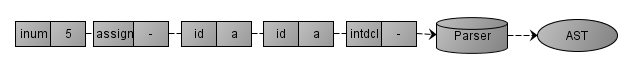
\includegraphics[scale = 0.5]{img/parser.png}
	\caption{Parser Phase}
	\label{fig:parser}
\end{figure}

\subsection{The Symbol Table}

The symbol table is a central table accessible from all compiler phases which, as mentioned, contains all identifiers and the information that is associated with these. When the declaration of an identifier is recognised by the type checker, it is stored in the symbol table along with its scope, type, so that the next time it is used it can be retrieved from the table.

\subsection{Type Checking}
The semantic analysis creates what is called a decorated AST. It checks what is called the static semantics of each node. This means that it checks that each node is meaningful and legal with regards to type etc. for the source language. If it is, the node is decorated with type information, e.g. an assignment node can be decorated with the information that it is an assignment of an integer. Should an error be discovered, for example assignment of a string to an integer, an error message is sent out. 

A type can be defined as "any property of a program that we can establish without executing the program" \cite{Krishnamurthi2007}. The definition of types varies from language to language, but common for all is the notion that types are a certain set of values, and some operations on these values, that behave the same every time the program is run. As an example a Boolean type has only the values true and false. 

The decorated AST of the example code is shown here:

\begin{figure}[ht]
	\centering
		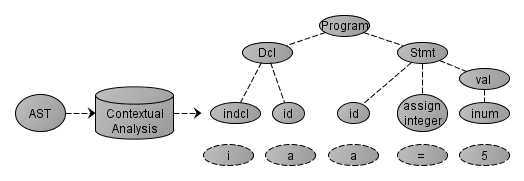
\includegraphics[scale = 0.6]{img/dast.png}
	\caption{Decorated AST}
	\label{fig:dast}
\end{figure}

\subsection{The Code Generator}
This is where the target code is generated from the decorated AST. This phase requires detailed knowledge of the target machine, e.g. register allocation, code scheduling and more. This phase is frequently coded by hand instead of using a tool, and a good code generator requires many special cases to be considered.

The final phase of the example code is shown here:

\begin{figure}[ht]
	\centering
		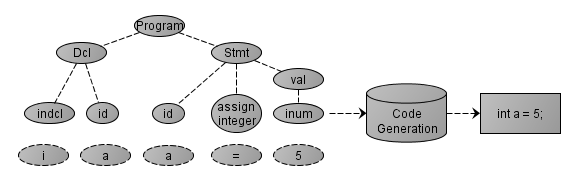
\includegraphics[scale = 0.6]{img/codegeneration.png}
	\caption{Code Generation}
	\label{fig:codegen}
\end{figure}

\section{Compiler Construction Tools}

  When creating a compiler for a programming language, several tools which can automate part
  of, or even the entire process, exist. These tools are split into parts that correspond to 
  the different parts of a compiler.
  
  \subsection{Scanner Generators}
  
    Scanner generators, such as Lex \cite{yacchome1}, require the user to create a set of rules
    for the tokens the compiler should recognize, often using some form of regular expressions,
    combined with what it should do for each of these tokens, often putting it on some form
    easily interpreted by a parser.
    \\
    Lex output c code which can easily be implemented in a complete compiler, with a function that
    generates tokens. It is up to the programmer to create, either by hand or using a parser
    tool, the functionality to handle these tokens.
    \\
    Ambiguous token definitions may or may not be handled by a scanner generated in this way,
    for example in Lex, if two rules match the current point in the input stream, it will
    choose the rule matching most characters. If the same amount of characters are matched,
    Lex will use the rule defined first.
    
  \subsection{Parser Generators}
    
    Parser generators, such as Bison \cite{yacchome2}, generates a parser for a language, using a
    context free grammar as input. The format of this context free grammar depends on the
    generator in question, in the case of Bison, something similar to Backus-Naur Form is used.
    \\
    Bison, like Lex, outputs c code with a function to parse a file. This function expects a
    scanner function, such as the one generated by Lex, to be present. Bison allows you to define
    actions for what happens with successful parsing of a grammar rule, in simple cases the parser
    may be enough to generate the desires output, but for most programming languages, a parser will
    build an abstract syntax tree for various semantic checks and code generation.
    
  \subsection{Full Spectrum Compiler Construction Systems}
  
    Some tools, such as Gentle \cite{gentlehome} allow the generation of an entire compiler, including
    scanner, parser, tree traversal and code generation. These tools requires input in the form of
    rule definitions, for tokens, grammar and actions, and output a compiler able to translate a source
    language into a target language.
    
  \subsection{Pros and Cons of Automation}

	For languages with a large amount of token and grammar rules, using automated tools, can save
	a lot of time compared to creating the tools by hand. Making adjustments in the language which
	require a restructuring of for example the parser, is less of an issue when a tool is able to
	generate a new one without much work being done.
	\\
	For a small language however, crafting a compiler by hand can be faster, since you do not have
	to learn the format of the input the tools need to work. Additionally, when hand-crafting a compiler
	it is possible do custom optimizations, like for example creating the parser from e human-readable
	grammar, instead of having to create grammar rules specifically to optimize the output of the tool.
	
    
%TODO References: yacchome: http://dinosaur.compilertools.net/
%TODO References: gentlehome: http://gentle.compilertools.net/
\section{Analysis of Role-playing systems}
Our target-group consists of people experienced in role-playing, both digital games and \emph{Pen \& Paper} games. Question sheets were created and sent out to a part of our target group, where questions regarding role-playing experience (number of known systems, years played, etc) and programming experience were answered. This helped us with designing our language to the needs of the target group.
After analysing the question sheets\vref{qsheets} we decided to take a closer look at three systems, described in the next section. The reason for this, is to find common characteristics and try to adjust our language to the basic needs of these popular role-playing games.

\subsection*{Role-playing games}

The World Of Darkness (WoD) is a supernatural horror role-playing game, which incorporates a system called \emph{Storytelling System} developed by \emph{White Wolf Inc}. It's world consists of mythical creatures like vampires, werewolves and ghosts. The system is unique in the way it handles character health and damage, which is categorising received damage and assigning a symbol to each type, making it easy to keep track of changes. The outcome of events is decided with one or more 10-sided dices.\cite{wod}

Dungeons \& Dragons (DnD) is a fantasy role-playing game, which incorporates a system called \emph{d20 System} developed by \emph{Wizards of the Coast}.
It's world consists of mythical creatures like elves, dwarves, dragons and other supernatural beings. The fact that the system is the first to be published commercially makes it an interesting reference. The outcome of events is decided with a dice pool containing 4-sided up to 20-sided dices, the 20-sided ones are used to roll for success (use abilities).\cite{dnd}

Cyberpunk 2020 (Cyberpunk) is a role-playing game with a postmodern science-fiction setting, which incorporates a system called \emph{Interlock System} developed by \emph{R. Talsorian Games}. It's world consists mostly of humans, cyborgs and robots.
The \emph{Interlock System} is skill-based instead of the traditional level-based system. Meaning that players get awarded points to spend on their skill sets instead of experience points. The outcome of events is decided with a similar dice pool to 'DnD, but using 10-sided dices to roll for success.\cite{cyberpunk}

\subsection*{Common characteristics}
\label{baseclasses}
The systems have some basic requirements to provide optimal playing experience, such as:
Character classes, attributes, effects, abilities, resources, modifiers and variation (dice rolls). These core entities represent their respective real-life concepts and the dice rolls introduce 'luck' to the mix.
Each of these systems have their 'dice pool' and their rules which define what types of dices and how many are involved in a given task.
The systems' dice size and quantity differ, but are derived from the same concept: \textit{''To decide the outcome of a given task, you must roll a dice of a specific size, add modifiers, calculate the result and compare to the task's difficulty. If your result is higher, you succeed''}\\

What these systems have in common, although implemented differently in each, is health points, damage and their calculations. This results in a different approach to our engine's damage calculations. While \ac{wod} and \emph{Cyberpunk} have some very convenient representations for \emph{pen \& paper} role-play, they are not suitable for our engine, reason being that health has various types, be it bashing, lethal or aggravated.
With this implementation the system captures some real-life forms of damage. An attack with a knife therefore does not have the same effect as with a hammer. Whereas in a health-resource based implementation, like in some video games, an attack does an amount of damage regardless of the type of attack. The amount is then subtracted from the health pool of the victim.
A character sheet from the game \ac{wod} is presented for reference on appendix \vref{charsheet}. As seen on the character sheet, a character is defined by their \emph{Attributes}, \emph{Skills} and \emph{Other Traits}. When playing a game, it is recommended to have the core rulebook as support, since calculations and various details about happenings is defined there.

\subsubsection*{Conclusion}
As a proof of concept, we choose the common characteristics of these systems for constructing the rulebook, common characteristics being the before mentioned \emph{requirements} of the systems.
By using Characters classes, attributes, effects, abilities, resources and modifiers, we can define a character in our language, like it was a character sheet. If done correctly, this should satisfy our target group.

\begin{comment}
\subsubsection*{''Final Fantasy'' \& engine specifics}
The Event system and fight simulation will be based on the first games of the video-game series \emph{Final Fantasy}, this is done to simplify the implementation. Final Fantasy is a fantasy role-playing game, released for the \emph{Nintendo Entertainment System} in 1987. The game was a success and has since then spawned a whole franchise named after the original title.
The Final Fantasy series have implemented various combat systems, turn-based and real-time.\cite{ffantasy}
Since our engine simulates battle and provides fairness through modifiers, we choose turn-based combat, where a battle is measured in turns.
For simplicity we also choose to restrict the number of contestants to two.
\end{comment}


%sources: WoD - The World of Darkness (ISBN: 1-58846-484-9) by White Wolf Publishing
%sources: Cyberpunk 2020: The Roleplaying Game of the Dark Future (ISBN: 0-937-279-13-7)
%sources: Dungeons & Dragons Player?s Handbook: Core Rulebook I, v. 3.5  (ISBN: 0-7869-2886-7)
%sources: Gameplay of Final Fantasy (http://en.wikipedia.org/wiki/Gameplay_of_Final_Fantasy)
\section{Language paradigms}
Within computer programming, a \emph{paradigm} is a model or framework for problem solving. \citeauthor{paradigms1992} describe it thus:

\begin{quote}
A programming paradigm is a collection of conceptual patterns that together mold the design process and ultimately determine a program's structure.
\end{quote}

The granularity with which paradigms are defined varies somewhat between sources. While \citeauthor{paradigms1992} keeps to the understanding that a paradigm is a larger philosophy of solving problems computationally, other sources maintain that a paradigm can be considered on the level of techniques (\citeauthor{paradigms1978} on divide and conquer \cite{paradigms1978}). Within the context of this report, we constrain ourselves to the more abstract form as presented by \citeauthor{paradigms1992} in order to better represent the higher levels of paradigms. The point of the discussion is to present an overview of the major paradigms, their main points of interest and perceived strengths/weaknesses of each. The discussion of paradigms is important, as choosing a proper paradigm (or set of paradigms) is key in considering how the target users should work with the designed language.

\citep{paradigms1992} put the paradigms into three categories: \emph{operational} (where programs are described as step-by-step procedures), \emph{demonstrational} (a higher-level abstraction where an example is shown and the compiler must derive a procedure from it) and \emph{definitional} (solution properties are described, but the method of solving it is not). The demonstrational paradigms lie beyond the scope of this project owing to its "code-by-example" approach, going close to (or within) the domain of graphical programming. It will not be further discussed.

\subsection{Operational versus Definitional}
To more easily narrow down the field of optimal paradigms, first consider the two overarching categories of the operational and the definitional paradigms.

In solving problems, the operational paradigms focus on specifying the solution method in sequencial steps. The granularity and focus of this approach is beneficial as solutions can be specified very precisely and the corresponding result sets are at the very least clear. However, it also demands a certain degree of familiarity with mathematical and algorithmic approaches to defining solutions, two disciplines not often found outside of programming. A necessary effect of this is the strict sequencing of steps, each one creating a new data state.

In contrast, the definitional paradigms focuses on constraining the solution set. As stated by \citep{paradigms1992}:

\begin{quote}
In definitional paradigms, a program is constructed by stating facts, rules, constraints, equations, transformations, or other properties about the solution value set.
\end{quote}

The programmer is no longer required to specify \emph{how} to reach a solution, only what a correct solution should look like. This can, in principle, alleviate some of the more complex aspects of programming tasks, making the language notably easier for beginners, hobby programmers or non-programmers. With from this assumption, we shift our attention only to the definitional paradigms.

\subsubsection*{Functional}
The functional paradigms focuses on the serial application of functions to reach a desired solution. The basic approach can be likened to mathematical function definitions. For example, the mathematical function

\[
f(x) =
\begin{cases} \frac{x+3}{12} & x \texttt{ mod } 3 = 0 \texttt{ and } x \geq 9
\\
\frac{x}{12} & x = 12
\\
(x * 4)^2 & \sqrt{x} = 3
\end{cases}
\]

Where the computation of the function is based on conditions related to the function argument. A similarly structured approach in a functional (pseudo) language could look like so (recall that $\sqrt[2]{x} = 3 \Leftrightarrow x = 3^2$):

\begin{lstlisting}
// The function f as defined equivalently above.
func f(X)
	:= (X+3)/12 if (X % 3 == 0 and x >= 9)
	:= x/12 if (X == 12)
	:= pow(x*4,2) if (x == pow(3,2))

// Function calculate power of a number.
func pow(I,P)
	:= I*pow(I-1,P) if P > 0
	:= I if P=0
\end{lstlisting}

There are several features of note in this approach. First of all, the deeply ingrained conditionals. A particular computation (in this case, a line of code) is performed only if certain conditions hold. Flow control (or line ordering) is a second feature (or lack of the same) to note. The functional paradigm can be applied in such a way so the order of conditions in a function are of no consequence. Indeed, this can be seen in the implementation of the $pow$ function. In an imperative recursive implementation of $pow$, the conditional check for $P==0$ must come before the recursive step as each line is evaluated downwards. This does not need to be the case for the functional approach. During evaluation, each line's conditions are checked. How and when branching is performed varies between implementations. Some short circuit (first match, if any), others with either most conditions met or most percentage of conditions met. The printed example assumes the latter. In all cases, a mechanism for defaults must be supplied as well. One approach is to use the last line if nothing holds. This would be considered an operational - imperative - approach, somewhat contrary to definitional dogma. Another would explicitly specify the default case.

The particular strength of the functional paradigms is the release from control flows and program states (note the lack of any intermediate or long-term variables) while attempting to adhere to mathematical principles for function definitions. It is left to the programmers of the compiler or interpreter to derive the proper execution order and result set. There remains, however, a need for the user of the language to understand fundamental discrete mathematics in order to properly apply the paradigm to a problem.

\subsubsection*{Transformational}
Transformational paradigms define a problem solution by a series of transformations. For example, the input $17$ might be transformed to $108$ through the transformations $17 \rightarrow 119 \rightarrow 108$ (using $17 * 7 = 119$ and $119 - 11 = 108$). A program is specified by a number of \emph{gourds} (conditions) and \emph{actions} (transformations) that define the possible transitions the input may go through. In this sense it has similarities with the functional paradigm. The difference, however, lies in how the transformations are applied. Where the functional paradigm leaves it to the programmer to specify which functions should be used, the transformational expects the system to identify which transformation to apply at any given point. In this manner, the system will transform the input until no guard will match it. At this point, the result is returned.

\subsubsection*{Logic}
The logic programming paradigm makes use of Horn clauses to describe predicates and the facts that must hold true for the predicate to do so as well. Horn clauses are beyond the scope of this report, but for context a brief example is in order. using notation of boolean algebra, a horn clause could be written as 

\[
(c_1, c_2, \cdots , c_n) \rightarrow f
\]

should be read as ''if the conditions $c_1$ to $c_n$ all hold true, then fact $f$ must also hold true''. A program written in the logic programming style is comprised solely of clauses like this. The programmer must define sufficient facts (and a goal to be reached), and the compiler must be able to deduce the correct resolution of facts to reach this goal. The set of possible combinations that must be tested to find the solution very quickly becomes so large that algorithms used for solving the problem must be heavily optimised, and even small changes to the ordering of facts can markedly affect the performance of the program. While several algorithms with acceptable running times have been designed, it still remains a challenge for the programmer not only to supply sufficient facts to deduce a solution, but also in a manner that is not counter-productive to the overall running time of the programmer. While the latter can be argued to be a staple of any programming paradigm, none would have as great an impact as in the logic programming paradigm.

\subsubsection*{Form-based}
Perhaps one of the simplest examples of the form-based paradigm in use is a spreadsheet application such as Microsoft Office or LibreOffice Spreadsheet. Computations are specified via equations, and can entirely avoid explicitly defining a control sequence by virtue of their interdependence. An equation must be computable independently of its result (that is, circular references are not allowed). Any formula $x = f(y_1, y_2, \cdots , y_n)$ therefore requires that all $y_i$ be computable independently from $x$.

This paradigm's strong point is the form in which programming is done. It is analogous to filling out regular forms (tax forms, applications - even character sheets) and should come naturally to many users - as a consequence, the roles of programmer and user become very close entwined.

\subsubsection*{Dataflow}
The dataflow paradigm regards input as a flowing stream of data, passed through nodes in a network that apply a formula to the data. The sequence is determined by the programmer as it is with the functional paradigm, but the dataflow philosophy is very well suited for parallel processing of data. Several streams of data may flow through nodes, and their paths may be independent before or after they pass the node. At those points, individual threads could handle each stream through other nodes until they converge. Conversely, each node could be handled by an individual thread, awakened whenever sufficient streams had entered the node for processing, and sent back to sleep when not needed.

\subsubsection*{Constraint programming}
This paradigm might best be described as the programmer's equivalent to an equation solver. The intention is for the programmer to sufficiently \emph{constrain} the solution's value set. This does not mean to simply write out formula for the system to evaluate given certain input, but to instruct the system as to how the formula remains valid. Consider an equation

\[
y = x^3 + 12c
\]

In the case of form-based, functional or dataflow paradigms, one would expect that $y$ could be computed once appropriate values $x$ and $c$ have been input. Constraint programming, however, should support finding any variable once enough of the other variables have bene passed. Consequently, the equation

\[
\sqrt[3]{y - 12c} = x
\]

is programmatically equivalent. The system must be able to derive these equations and computational possibilities on its own, without the programmer (assuming the programmer properly constrained the problem).
\pagebreak
\section{Syntax theori}
% ~Hornbjerg
Every language, whenever it is English, German, or some other language, have some specified gramma, used for making sentence in the languages. The gramma of the languages is specified by rules, which desripe how to use the gramma corretly.   \\
Every sourcecode of a program, written in some programming language also consist of some sentence. Specify how a correct sentence in programming languages i written, the programming language uses a set of rules called the \textit{syntax} of the language. The syntax of a programming language can be descriped i deffirent ways, but in this section, we focus at three ways:
\begin{itemize}
\item{\ac{cfg}}
\item{\ac{bnf}}
\item{\ac{ebnf}}
\end{itemize}

\subsection{\ac{cfg}}
\ac{cfg} was first descriped in the middel of the 1950s by Noam Chromsky. A \ac{cfg} is a colloction of substitutions rules. The rules consist of two kinds of symbols; \textit{nonterminals} also know as \textit{variable} and \textit{terminals}. Each rule in a \ac{cfg} is formed as a line, which constist determents how substitut one (ore more) \textit{variables} with an other vaiable or terminal. \\
An example of a \ac{cfg} is 

\begin{tabular}{l l l}
$A$ & $\rightarrow$ & $0A1$ \\
$A$ & $\rightarrow$ & $B$ \\
$B$ & $\rightarrow$ & $\#$ \\
\end{tabular}

In the gramma above the rules shows that $A$ can be substituted by either $0A1$ or $B$. \\
The \ac{cfg} above will be called $G$, and the language which can be generated by the \ac{cfg} $G$ is called a \textit{context-free language} and is written $L(G)$, which means $L$ is generated by $G$.

\subsection{\ac{bnf}}
In 1959 a new formal notation used to specify the syntax of at programming language was introduced by John Backus, and the notation was later modified by Peter Naur, and the notation was called \ac{bnf}. \\
\ac{bnf} is an other way of descriping syntax of a programming language. Like a \ac{cfg}, a \ac{bnf} is a collection of rules, which also uses \textit{terminals} and \textit{nonterminals}. An example of \ac{bnf} used to descripe a simple Java assignment statement is written as

\begin{tabular}{l l l}
$<\texttt{assign}>$ & $\rightarrow$ & $<\texttt{var}> \; = \; <\texttt{expression}>$ 
\end{tabular}

where $<\texttt{assign}>$ is an abstract reprecentation of an assignment statement, and the rule specifies that $<\texttt{assign}>$ is defined as an instance of the abstraction $<\texttt{var}>$ followed by the `=' symbol, and then followed by the abstraction $<\texttt{expression}>$.

\subsection{\ac{ebnf}}
\ac{ebnf} is an extended version of \ac{bnf}. The \ac{bnf} has though time bin extended i several ways, and even though all the extenssions is not exactly the same, the are all called \ac{ebnf}. The extensions only makes the notation more readable and writeably, they does not enhance the descriptive power of \ac{bnf}. \\
One of the things included in one of the extensions of the \ac{bnf}, denotes an optional part at the right-side of the ``$\rightarrow$'', which is delimeted by brackets. for an example, an \textbf{\texttt{if-else}} statement, in the programming language C. The statement can be descriped

\begin{tabular}{l l l}
$< \texttt{if\_stmt}>$ & $\rightarrow$ $ \textbf{\texttt{if}} \; ( < \texttt{expression} > ) \;  < \texttt{statement} > \; [ \textbf{\texttt{else}} \; < \texttt{statement} > ]$
\end{tabular}

With use of \ac{bnf} the statement would be desriped \\

\begin{tabular}{l l l}
$< \texttt{if\_stmt}>$ & $\rightarrow$ &  $\textbf{\texttt{if}}  \; ( < \texttt{expression} > ) \;  < \texttt{statement} >$ \\
 & $|$ & $ \textbf{\texttt{if}} \; ( < \texttt{expression} > ) \;  < \texttt{statement} > \; \textbf{\texttt{else}} \; < \texttt{statement} > $
\end{tabular}

% 3. Language definition.
\chapter{Language Definition}
\section{Language constructs}
The \langname{} language has resulted in a highly declarative style of programming, focusing on what is to be done, but not how. Several of the concepts featured in the language have well-known parallels in other programming languages e.g. events/signaling, classes, inheritance, user-defined types, the concepts have been modified to specifically target the domain of role-playing games.

The very first iterations of \langname{} presented a hybrid attempt between the implicitly understood effects of declarative programming with the flow control of imperative programming. After analysing the target audience, it became clear that the language should provide for simplistic input of objects and their relationships, without the hassle of considering line ordering or algorithms. The focus should not be on having the programmers define the rule-sets and calculations of the games \cite{wod}, but rather let them take the natural role of a \ac{dm} and define not the world, but its contents. This has resulted in the unavoidably imperative elements of the language. In particular the rule set and base derivations of types, which have be segregated into pre-written $C++$ code, while the definition of characters and the setting of their attributes remains within \langname{}. This section describes the primary features of the \langname{} language as well as the underlying reasoning behind them.
%\todo{classes?} \todo{change if we go higher/lower} % Done
\subsection{Paradigm}
\label{language:paradigm}
\langname{} has taken on traits of declarative programming languages that focuses on letting the programmer describe \emph{what} they want, but not necessarily \emph{how}. It is evident in the three basic interaction methods in the language: \emph{declaration}, \emph{assignment} and \emph{construction}. All three are demonstrated in the following snippet. \todo{Double check the syntax for Fireball.Costs - I can't remember how we referenced members like that.}

\begin{lstlisting}[language=fflang]
make Fireball from Ability
{
	Costs: [[user.Resources[Mana],-10]];
	Targets: [all];
	Effects: [
				[FireDamage(10,target)],
				[FireDot(3,3,12)]
			];
}
\end{lstlisting}

The user-defined type of Ability, in this example called \emph{Fireball}, is declared and its members are assigned the necessary values. Notice the syntax for each of the effects ($<EffectName>(<param_1>, \cdots ,<param_n>)$), reminiscent of procedure calls in many other languages, and indeed the best equivalent would be that of a class constructor. This code is all that is necessary in order to implement Fireball into the game and make it available to characters.
While not strictly adherent to any single rule system, each base type in the language models a particular part of systems that was deemed almost universal across those reviewed. For example, many abilities of characters have a cost associated with them, especially magic abilities like Heal, which replenished HP. %TODO: Acronym?
%As an example, 4th edition of \ac{dnd} limits the number of times an ability, can be used as a number of times per game day, encounter (battle) or ``at will'' (without restriction). Both types should be possible with the generalised assignment method and should thus cater to many different systems \todo{Test/confirm/analyse/look}. All other base types contain similar members (see the language reference for full descriptions).
The type members and the method of declaration attempts to mimic the filling out of character sheets (see appendix \vref{charsheet} for an example) in pen and paper role-playing games. When a player or \ac{gm} fills out a character sheet they will, line for line, write the values for the character in appropriate fields. These are erased and updated as necessary, for example, when the character takes damage.
Likewise, the programmer details the character as they should appear at the beginning of a battle according to a pre-defined rule set, which defines which types of Attribute, Resources and Effect are available during a battle.
%This philosophy data-driven programming is further described within the context of several key areas of programming in the following sections. % Done
\subsection{\langname{} Rule Set}
\label{language:ruleset}
Many systems have complex conditions or calculations for some of their aspects.
Analysing the target group's most popular systems, rules were exposed that cannot be easily expressed in a generalised declarative manner.
An example is the health system of the revised Storyteller system from the \ac{wod} series of games. Three distinct types of damage cover the same seven points of health. Damage must be calculated on specific areas of these points, and have different healing times.
Simpler examples of rules are damage calculations in most video \ac{rpgs},
where certain attributes will lower the damage sustained from specific categories of damage. In Final Fantasy I, which is the rule set used as a guide for stats, physical attack damage is determined from two formulae depending on the active character's class. Below is the calculations implemented in the engine, as it is evident this is an almost exact copy the attribute calculation from Final Fantasy I:

\subsection{Implemented set}
\label{language:implset}
\begin{center}
\begin{tabular}{|l l l|}
\hline
\multicolumn{3}{|c|}{\textbf{Attributes}}\\
\hline
Strength: & Manually Set & (used for Damage calculations)\\
\hline
Agility: & Manually Set	 & (used for Defense calculations)\\
\hline
Intelligence: & Manually Set & (used for Mana calculations)\\
\hline
Stamina: & Manually Set & (used for HP and Defense calculations)\\
\hline
\end{tabular}\\
\emph{All the above listed attributes are manually set by the programmer.\\ These initial values are fundamental for a character in the implemented world. If the programmer does not set these, they are initialized with the value 0.}
\end{center}

\begin{center}
\begin{tabular}{|l l|}
\hline
\multicolumn{2}{|c|}{\textbf{2nd Attributes (calculated)}}\\
\hline
Defense: & ((Stamina + Agility) / 3)\\
\hline
Magic Defense: & ((Stamina + Intelligence) / 3)\\
\hline	
\end{tabular}\\
\emph{These second attributes are calculated with the given values of the initial attributes.\\ They serve as defense for the two damage types, by subtracting their calculated values from the damage taken.}
\end{center}

\begin{center}
\begin{tabular}{|l l|}
\hline
\multicolumn{2}{|c|}{\textbf{3rd Attributes}}\\
\hline
Attack Power: & (WeaponDmg + ((Strength / 2) + 1))\\
\hline
Magic Power: & (Equipment bonus + ((Intelligence / 2) + 1))\\
\hline
\end{tabular}\\
\emph{These values are calculated from the manually set attributes and calculate damage.}
\end{center}

\begin{center}
\begin{tabular}{|l l|}
\hline
\multicolumn{2}{|c|}{\textbf{Resources}}\\
\hline
Health Points: & (Stamina * 20)\\
\hline
Mana Points: & (Intelligence * 15)\\
\hline
\end{tabular}\\
\emph{These are the Resources most often used in RPG systems. They represent physical health and magical energy respectively. Mana is the cost of Abilities.}
\end{center}

Additionally, it was decided that for simplicity a character would die, i.e. leave combat, once their HP reached 0. Also, due to the fact that Items were never included mana replenishing items such as mana potions are not available. This means that mana is a depleteable resource. It was also decided that a character wins combat if they are the only one still alive. % Done
\subsection{Program control and structure}
Program control and control structures refer to the mechanisms in a programming language that allow a programmer to define the order of execution of the code as well as conditional branching into subregions or even looping. \langname{} has almost none, going so far as to be completely order-agnostic with line ordering in-scope. 
%\todo{Bad guess: our language is declarative, yes, and perhaps more specifically a functional derivative. While we have very little in the form of functions (see Effect()), we apply our assignments in basically the same manner. One could consider the assignment of values to members equal to the passing of function arguments, and the declaring of types to be the function calls themselves.}
The form-filling tendencies of the language are quite evident in this aspect. While a strict line ordering would better serve the metaphor, the loose ordering %is simpler for a compiler to parse \todo{Are we sure that is true?} (avoiding an unknowable number of extra passes required for a proper semantic analysis) and 
affords experienced programmers to lay out their code as they choose according to readability. %As a consequence, there are no conditional or iterative control structures. \todo{Can I rationalise this?}
The reasoning for this design choice stems from the target user group. While not necessarily a complex task, the algorithmic design activities involved when applying control structures to a problem are not commonplace within the role-playing community. Instead of forcing down a framework for conditional reasoning over the users, \langname{} instead moves these principles into an predefined rule set.
%If specific conditions change the state of a character, or their definition relies on the iterative execution of logic, it is handled externally and passed into the final character as necessary by the Engine.
A goal of the language design is to keep it sufficiently simple for novice programmers (and non-programmers) to work with, conditionals would primarily increase the amount of work involved in defining the battle. %If they were to be introduced in \langname{}, the users would also need to work with object references, signaling and inheritance.
%This is due to the fact that anything that modifies a value in transition from one character to another (for example, damage) must be handled by the engine. If the programmer wants to catch and modify this, they must register for appropriate events, reference involved characters, modify the transition value according to the rules and send it back into the pipeline. The code could further be improved if this was handled in a subclass of the appropriate \langname{} base class. Thus it is not enough to simply introduce the necessary language construct.
%Instead, the rule set is specified externally as a subclass of the Engine-defined RuleSet class 
%\todo{reference documentation and/or name/architecture check} 
%(see \\ref\{wherever\}) programmed in $C++$, and used as a reference by the Engine when running the simulation. % Done
\subsection{Types and user-defined types}
\label{language:types}
The core concepts of any roleplaying game necessitates a very rigid data structure, and the basis for \langname{}'s reference rule set is no different.
\langname{} defines a number of generalised base types, derived from the concepts found through most of the \ac{rpg} systems analysed. They are, briefly, as follows:
\begin{description}
	\item[Character] defines any acting entity with an invididual turn sequence.
	\item[Resource] Represents values, like health or mana, that can have a minimum and maximum value.
	\item[Attribute] Represents any numeric value associated with the Character, this could be; Strength, Intelligence an so on.
	\item[Behaviour] sets the values used to calculate a decision tree for a Character.
	\item[Event] represents a reactive AI routine. Complements Behaviour.
	\item[Ability] is any action known to a Character.
	\item[Effect] types are associated with Ability types and define what happens when an Ability is used.
	%\item[Item] describes consumable or equippable items in the game, that may rise the current value of an Resource or Attribute, such as a sword or a potion.
\end{description} 

All of the types except Event and Behaviour were derived from the combined concepts of the systems analysed. All the systems contain Characters with core characteristics (Attributes and Resources). Depending on their archetype (or class or equivalent \ac{rpg} concept), the Characters have differing sets of abilities.
Abilities have the capacity to affect the game in some way (Effects), although they will not always be successful or fully potent (see \vref{language:ruleset}). An Ability will almost always have an associated cost. If not time (a turn), some resource must be expended in order to execute the Ability, for example Mana. %Finally, Items are an almost universal feature, either in the form of useable objects (which, in turn, expend some form of resource of the Character or the Item) or as an equippable (a sword, a helmet, a ring or similar).

Event and Behaviour are defined as a means for the programmer to describe how Characters should act within the scenario. While it is very rare for a pen \& paper rulebook to describe character behaviour in full play by play, they do often describe character traits that can be used to derive behaviour. This description is necessary for a later AI simulation to make meaningful decisions (see the AI section \vref{analysis:action}). %\todo{Write that section...}).
Conversely, most if not all, video \ac{rpgs} demonstrate some form of AI in NPC's.

In order to make use of the types, the programmer must define a named version of that type. Although it is difficult to define this mechanism as either instantiation (object of class) or inheritance (subclass of class), it mostly resembles the prior. The programmer must define a type (say, a new Ability - Fireball) strictly following the data structure of its source (Ability). \langname{} does not support extending the structure of any type. For example, the Fireball Ability cannot add a member named "colour". It is, however, possible to further derive from a named type (creating a BigFireball from Fireball, for example) wherein selected member values can be modified to create a similar Ability but with a slightly different flavour. Another trait evident from this type derivation (and member assignment) is that type names and variables go into one. Once the Ability derivatives Fireball and BigFireball have been declared, they can be inserted into a Character's Ability collection via assignment.

The reasoning falls back to the targeted end-users and the focus of creating simple constructs with enough flexibility to define desired combat scenarios. Named variables are unnecessary as no more than one instance of any specific derivative was found to be necessary, multiple consumable items was a possible consideration, and an Item archetype was discussed to encompass these, but never described syntactically due to time constraints.
%The resulting localised Singleton pattern or nameless object (while Fireball is only defined one place, each occurrence on a new Character constitutes an individual instance) much closer resembles the typical method of filling out data in a character sheet - it is very rare indeed to see a system where the player is required to come up with their own name for an Ability, not least because it makes the \ac{dm}'s task much more complex, and needlessly so.
 % Done
% \emph{make} allows for the inheritance from the adjusted core classes (called primarchs) of the base framework. While the Primarchs encompass several qualities often associated with object-oriented paradigms (encapsulation and inheritance), they also exhibit traits that detract from such a broad definition. In particular, primarchs and their seeds \todo{Find a better word for "children"} are highly specialised from their core, created for particular purposes within our bounded RPG framework \todo{Reference Biggi's analysis and ruleset}. Furthermore, Primarchs support no notion of class procedures, explicit instantiation or structural extendability. Any seed cannot change the first-level membership structure of its parent (it cannot add new members to the immediate structure, only modify existing members). Finally, \langname{} does not support variables of any form. Any additions to a declaration happens by name of the type and nothing else. Note, however, that this is by no means a singleton pattern approach. While members of a Primarch are referenced by their type name, not an arbitrary variable, the code does not reference a static class, rather a nameless instance bound to the Primarch in question. The following is a list of the Primarchs inheritable within \langname{} files:

\subsubsection{Character}
Defines any individual participant in the battle scenario. These are the root containers or associative centers for all other classes. While the Character primarch references the character's definition, it relies on the definitions of contained seeds of other primarchs to actually define it.

\subsubsection{Behaviour}
Details how a character's attributes and resources should be weighed according to each other as well as those of other characters. These weights define the character AI's "Piggy" value when calculating most beneficial actions mid-game. This forms half of the exposed mechanisms for modifying AI logic in \langname{}, the other half being Events. 

\subsubsection{Ability} 
Key to describing a character's set of possible actions. Any action taken by a character will be described by an ability, from swinging a sword to weaving intricate spells and drinking potions. A seed of Ability defines the name, cost, possible targets and associated Effects of the ability. For example, swinging the sword may be accompanied by a PhysicalDamage Effect that defines how the ability will affect the game state.

\subsubsection{Event}
Events are largely analogous to the signaling features of many other languages (see events in C\#, Java, $C++$ and others) in that they are logic structures that register themselves to be notified when (or if) a particular state is reached. Once notified, the event reacts with appropriate action. In \langname{}, Event primarchs are as declarative as any other primarch, and thus follows a very strict mechanic. Each Event defines a trigger for the event (known as a signal in the observer pattern) as well as an optional set of conditions that must hold for the event to follow through (for example, a Warrior's Blood Rage might trigger when the character drops in health, but only if he drops below $20\%$). Finally, the Event assigns a set of Ability references that will be attempted in sequence on the Character's next turn. Thus the Event primarch is the reactive half of the exposed mechanisms for defining AI behaviour (the other being Behaviour).

\noindent The following is a list of Primarchs are referenced (and initialised) within other Primarchs, but must be defined within the external ruleset (see \vref{ref_external_rulebook}).

\subsubsection{Resource}
For values that can vary within a range. The primary example of a resource is the notion of health for a character, described as HP (Health Points or Hit Points). A resource defines a base value, a current value as well as maximum and minimum boundaries. Typically, resources are used as basis for winning conditions (reducing an enemy's health below a minimum limit, killing him).

\subsubsection{Attribute} 
In contrast to a resource, an Attribute is a single numeral without boundaries. An attribute would typically be applied when describing the strength, dexterity, intelligence or other simply denoted value for a character. These values are not expected to fluctuate like Resources, although they are by no means constant.

\subsubsection{Effect}
Must be contained and associated to Abilities. Each defines the result of applying an Ability to a target by a Character. Effects are unique in the current design \todo{Delete if irrelevant} in that they are the only primarch with a trait akin to a class constructor.

\noindent As described, primarchs have widely different uses, but are tightly connected to each other in order to discretely and precisely define the battle scenario by the programmer. They share no common ancestor, as they are each treated specially by the Batteru engine, revolving around the Character primarch. When a character's turn starts, the engine uses Behaviours associated with a Character to determine which of its known Abilities would result in the most beneficial game state. This is done by simulating the use of each Ability (applying the Ability's Effects) on every valid target and measuring the resulting Piggy value.

\emph{make} is the mechanism by which a primarch or seed is further specialised from its previous purpose. This is roughly equatable to inheriting in traditional object-oriented languages. \emph{make PhysicalDamage from Effect} creates a new Effect seed with all the defining features of Effect, while allowing the modification to the prior's definition.
 
% \subsection{Ranges and random values}
The language has built-in support of random number generation, going so far as to allow variables with unknown actual values until they are used in an expression. These types were conceived to cater to the widely used concepts of dice throws and resources. Resources are quite often described with minimum and maximum values. Dungeons and Dragons, for example, define a character's minimum and maximum health points as a factor of their chosen profession (class) and Constitution attribute (a measure of physical endurance). Likewise, damage rolls (the combination of dice and modifiers used to calculate damage dealt from an attack) are formulated in the general form $xdyy+z$ where $x$ is the number of $yy$-sided die to roll, plus a constant $z$, determined by modifiers relevant to the roll (strength for melee, intelligence for magic, for example). These calculations and types of data are somewhat trivial to implement in imperative languages, but the sheer frequency of their use invites a vastly simplified syntax for the expression of the concept. 	Consider the following example: a damage roll defined as $3d8+2$ in C:

\subsection{Inclusions}
A feature of Primarch and seed definitions, inclusions is a notation to define a member of a Primarch without explicitly instantiating with an identifier. An example:
\begin{lstlisting}[language=fflang]
make Attack from Ability
{
	targets: [enemy];
	effects: [	PhysicalDamage(target,12)
			 ];
}

make Cure from Ability
{
	targets: [self];
	mana_cost   : 7
	effects: [Heal(target,28)];
}

make BattleMageBehaviour from Behaviour
{
	positive : [[owner.health, 70]];
	negative : [[enemy.health, 80]];
}

make Wizard from Character
{
	abilities : [Cure, Attack];
	behaviour : BattleMageBehaviour;
	events    : [ ];
                 
    strength: 8;
    agility: 8;
    intelligence: 21;
    
    health: 80;
    mana: 100;
}
\end{lstlisting}

In this example, Wizard is made from the Primarch Character, and is assigned new abilities, values of attributes and resources as well as a behaviour. Notice that unlike imperative languages, only the identifier is given - no types are necessary, since each entry of the type is considered unique: It is impossible to have two Strength attributes on the same character. % Done 
\subsection{Relative Global References}
RGR's (or "RoGeRs") are a set of keywords that correlate to a dynamic set of global references. these are \emph{owner} \emph{enemy} \emph{target} to name a few, and will always reference the respective entity from the perspective of the local scope. \emph{enemy}, for example, will always reference the \textbf{other} Character in a battle when applied inside a Character subtype or its members, while \emph{owner} always references the topmost Character in a membership hierarchy. Consider the following code:

\begin{lstlisting}
make Fireball from Ability
{
	// Several mandatory members omitted for clarity.
	cost: [[owner.Mana, 10]];
}

make Wizard from Character
{
	abilities: [Fireball];
}

make Mage from Character
{
	abilities: [Fireball];
}
\end{lstlisting}

\emph{owner} when referenced in Fireball, will point to whichever Character is considering the ability. If it is the Wizard's turn and is calculating the use of the Fireball ability, \emph{owner} points to Wizard, not Mage. Essentially, this syntax approach wraps a parent-child relationship between objects (the hierarchy structucal design pattern) without the programmer having to specify these relationships explicitly. All of the RGR's thus automatically represent this relationship model, allowing the programmer to focus purely on the subtype at hand rather than the larger class architecture and the implications of n-element aggregation chains.
 % Done
\subsection{Summary}

The reasoning for this minimalist approach is three-fold: Firstly, it results in increased writeability and readability from the reduction of identifiers that need document referencing and memorization. Secondly, it vastly simplifies the style of writing for the definitions, much closer matching those of the character sheets that inspired them. Finally, the meticulous syntactical design creates a basis from which a much simpler language syntax is possible.% allowing for an efficient compiler construction. % Done

The programming language `RPG-script' is specifically developed for defining RPG(Role Playing Games) characters and abilities, attributes, resources, items and behaviour belonging to a character and the user of the language can define events, which are triggered by some conditions and uses some ability and finally the user can define that an ability triggers some rulebook defined effect. . 
In addition to the programming language is a game engine, which will simulate a turn based fight between the characters defined in the language. The engine also a predefined rulebook, where the core rules of the RPG-system is defined. 

The behaviour of a user defined character is A.I.(Artificial Intelligence) based, which means it is based at a value called \emph{piggy rate}, the character will consider its possible moves, and by an user defined priority, decide the move that will give the character the highest piggy rate at the end of the turn.

\section{Language syntax}
This section focuses at describing the general syntax of the `RPG-script' languages. The description will include a comparison of the `RPG-script' language and the `C++' language, in specially the parallels between inheriting of classes in the two programming languages. 

\subsection{Classes}
As mentioned above, the rules of the RPG system matching the `RPG-script' language is defined in the game engine, used for simulation a fight between characters.
Defining a character in the `RPG-script' language, is like inheriting a class in C++.
Lets see an example of inherit in C++:
\begin{lstlisting}
	class Animal
	{
		//Some members are put here
	}
	
	class Cat :: Animal
	{
		//Some members are put here
	}
\end{lstlisting}
In the example above the class \emph{Cat} inherit from the class \emph{Animal}. In the `RPG-script' language, the class, which is to inherit from is hard coded and the user may therefore define classes to inherit from, instead the definition of a class is an inheriting from the base classes; \emph{character, ability, attribute, resource, item, behaviour}.
Inheriting in the `RPG-script' language two keyword are used; \emph{make} and \emph{from}
\begin{lstlisting}
	make Human from Character
	{
		//Some members are put here
	}
\end{lstlisting}
In the example above the `class' \emph{Human} inherits from the predefined `class' \emph{Character}.
\subsubsection*{Members in classes}
Like in the C++ language, it is in `RPG-script' possible to make members of a class by enclosing the members in a block, by using the symbols ``\{'' and ``\}''.
\begin{lstlisting}
	class Animal
	{
		string name;
	}
\end{lstlisting}
In the example above, the class \emph{Animal} has the member \emph{name} which is a string, and the line is ended by the symbol `;'.
In RPG-script, the members are declared as collections, by using the symbols ``['' and ``]'', and separate the members of the collections with a comma `,', and ending the line 
\begin{lstlisting}
	make Human from Character
	{	
		Abilities:
			[ Pray, 
				Heal,
				Attack ];
	}
\end{lstlisting}
The example above makes a \emph{Human} class, with its members, which is a collections of abilities.
\subsubsection*{References}
In Object-Orientated programming languages, it is possible to make references to the classes, with the keyword \emph{this} and the operator \emph{->}. 
To define a character in the language, the user makes some primarchs, which is superclass, which not inherit from any other classes \todo{Primarchs are a type of primitive (basest of base classes), the real implementation of which is based on the external ruleset file}. The primarchs will be used for defining characters, abilities, attributes, resources, items, behaviours and effects.
Each primarch have members which may be references to an other primarch. The members of the primarch is enclosed in a block by using the symbols ``\{'' and ``\}''. To define a primarch the keyword \emph{core} is used \todo{Outphased. All "core" Primarchs are defined externally, and RPG-script exclusively defines the subtypes/inheritance}.
Let's consider the following code example 
\begin{lstlisting}
	core Character //Make a primarch called Character \emph{character, ability, attribute, resource, item, behaviour}
	{
	}
\end{lstlisting}
The code example above, makes a primarch with the name `Character'. 
To make member of a primarch, or class, a collections is used, which is declared by using the symbols ``['' and ``]'', and separate the members of the collections with a comma `,'.
\begin{lstlisting}
	core Character
	{
		Attributes:
			[ FireBall, //Make a collections of attributes as a member of the primarch
				Heal,
				Attack ]; 
	}
\end{lstlisting}
\emph{Fixed version here.}
\begin{lstlisting}
	make Wizard from Character
	{	
		// Attributes: // attributes, together with resources, are now defined exclusively in the external ruleset.
		Abilities:
			[ FireBall, //Make a collections of attributes as a member of the primarch
				Heal,
				Attack ]; 
	}
\end{lstlisting}
Because whitespaces has no function in the `RPG-script' language there is no deference between writing the code above, or writing:
\begin{lstlisting}
	core Character
	{
		Attributes:[ FireBall, Heal, Attack ];
	}
\end{lstlisting}
\begin{lstlisting}
	make Wizard from Character
	{
		Abilities:[ FireBall, Heal, Attack ];
	}
\end{lstlisting}
The language allow the user to inherit from a primarch or an other class, e.g. if the user want to make a `FireBall' ability, it can be made as a subclass of the primarch `Ability'. To inherit from a primarch, or an other class which not is a primarch, two keywords are used; \emph{make} and \emph{from} \todo{ALL inheritance is done this way, and only Primarchs (and their subtypes) can be inherited :)}.
Let's consider the following code example
\begin{lstlisting}
	make Strength from Attribute //Makes a subclass of Attributes which is named Strength
	{
		//Set relevant modifiers et al for this attribute.
	}
\end{lstlisting}


\section{Language semantics}
The language is a language used for  of a role-playing characters. I addiction to the language is an battle engine, which simulates a battle between the  character. \\
The engine works, so that lets one character make an action, then the turn end, and the other character then gets to make its action. \\
The action a character makes, is calculated by an AI-behaviour. The AI-behaviour is base at a behaviour declared for the character. \\
Before a character gets to make its turn, win condition is checked, so that the character does not get to make an action if its health is below zero.  

\subsection{Environment-store model}
The semantics of the language is base at the environment-store model, which is a a model describing how variables are bound during a program execution. Each variable is bound to a storage cell, and the content of the storage cell is the value of the variable.

\subsection{\langname{} semantics}
Five parts are highlighted for semantic description, these are  \emph{Declaration}, \emph{Turn}, \emph{AI}, \emph{Action} and \emph{Wincon}.\\
The first one 'Declaration' is the main function of \langname{} and the four that follow are not included in the language itself but in the engine.
A turn is a character takes an action, based at the outcome of the AI calculation \\
AI is calculation, which simulates every possible outcome, based on the possible actions a character can make. \\
Action is an event, which will make change for the stored values of the enemy character, or the character itself.\\
Wincon is a conditional check to see if the \emph{winning condition} is met.\\\\

The semantics for the relevant parts of \langname{} are defined as follows:
\begin{itemize}
	\item $EnvD$ is a declaration-environment
	\item $env_{D}$ is an element in the set $EnvD$
	\item $EnvC$ is a character-environment
	\item $env_{c}$ is an element in the set $EnvC$
	\item $StoreS$ is a set of locations and their bindings
	\item $sto$ is an element in the set $Stores$
	\item $Pending$ is a list of pending characters
	\item $ActioN$ is a set of available actions
	\item $act$ is an element in the set $ActioN$
\end{itemize}
\pagebreak
The rules for the five parts are as follows:
\begin{center}
\begin{tabular}{ c }
\textbf{Declaration}\\
\hline
 \\
$\langle env_{D}, env_{C}, sto \rangle \rightarrow$\\
$\langle env_{C}', sto' \rangle$\\
\end{tabular}
\end{center}
The transitions system for declarations is $(\Gamma_{DV}, \rightarrow_{DV}, T_{DV})$, whose configurations are defined by \\
\begin{tabular}{l l l}
$\Gamma_{DV}$ & $=$ & $(EnvD \times EnvC \times StoreS) \cup (EnvD, StoreS),$ \\
$T_{DV}$ & $=$ & $EnvC \times StoreS$ \\
\end{tabular}
\begin{center}
\begin{tabular}{ l l }
\multicolumn{2}{c}{\textbf{Turn}}\\
\hline
 & \\
$\langle Pending, env_{C}, sto \rangle \Rightarrow$ & \\
$\langle Pending', env_{C}, sto \rangle$ & $\text{if wincon } \rightarrow_{b} ff$\\
 & \\
$\langle Pending, env_{C}, sto \rangle \Rightarrow$ & \\
$\langle Pending, env_{C}, sto \rangle$ & $\text{if wincon } \rightarrow_{b} tt$\\
\end{tabular}
\end{center}

The transition system for turns is $(\Gamma_{TURN}, \Rightarrow_{TURN}, T_{TUNR})$, whose configurations are defined by\\
\\
\begin{tabular}{l l l }
$\Gamma_{TURN}$ & $=$ & $(Pending \times EnvC \times StoreS)$ \\
$T_{TURN}$ & $=$ & $(Pending \times EnvC \times StoreS)$\\
\end{tabular}

\begin{center}
\begin{tabular}{ c }
\textbf{AI}\\
\hline
 \\
$\langle Pending, env_{C}, sto, Action \rangle \Rightarrow$\\
$\langle Pending, env_{C}, sto, act \rangle$\\
\end{tabular}
\end{center}
The transition system for AI is $(\Gamma_{AI}, \Rightarrow_{AI}, T_{AI})$, whose configurations are defined by \\
\begin{tabular}{l l l }
$\Gamma_{AI}$ & $=$ & $(Pending \times EnvC \times StoreS \times ActioN)$ \\
$T_{AI}$ & $=$ & $(Pending \times EnvC \times StoreS \times ActioN)$ \\

\end{tabular}
\begin{center}
\begin{tabular}{ c }
\textbf{Action}\\
\hline
 \\
$\langle env_{C}, Pending, sto, act \rangle \Rightarrow$\\
$\langle env_{C}, Pending, sto', act \rangle$\\
\end{tabular}
\end{center}
The transition system for Action is $(\Gamma_{ACT}, \Rightarrow_{ACT}, T_{ACT})$, whose configurations are defined by \\
\begin{tabular}{l l l }
$\Gamma_{ACT}$ & $=$ & $(Pending \times EnvC \times StoreS \times ActioN)$ \\
$T_{ACT}$ & $=$ & $(Pending \times EnvC \times StoreS \times ActioN)$ \\

\end{tabular}
\begin{center}
\begin{tabular}{ l l }
\multicolumn{2}{c}{\textbf{Wincon}}\\
\hline
 & \\
$\dfrac{env_{C} \vdash c \rightarrow_{h} h}{\text{win} \rightarrow_{b} ff}$ & $\text{if } h > 0$\\
 & \\
$\dfrac{env_{C} \vdash c \rightarrow_{h} h}{\text{win} \rightarrow_{b} tt}$ & $\text{if } h \leq 0$\\
\end{tabular}
\end{center}
Wincon is special, because it is a boolean expression. \\
The rules evaluates true, if the demanded character $c$, has health evaluating to the value $h$, and the value is less or equal to zero, else et evaluates false, and the game will the continue 
\pagebreak

	$D_C ::= character C \{ D_A, D_R, D_B \}; D_C | \varepsilon$\\
	%D_C is a declaration of a character
	$D_A ::= A: v; D_A | \varepsilon$\\
	%D_A is a declaration of an attribute
	$D_R ::= R: v; D_R | \varepsilon$\\
	%D_R is a declaration of a resource
	$D_{AB} ::= AB \{ List[Rgr], List[effects], cost_h, cost_m \}; D_{AB} | \varepsilon$\\
	%D_{AB} is a declaration of an ability
	%cost_h is health cost
	%cost_m is mana cost
	$D_B ::= positiv | negativ : [Rgr.member, v]; D_B | \varepsilon$\\
	%D_B is a declaration of a behaviour

	
	$D_C \in Env_C$\\
	$D_A \in Env_A$\\
	$D_R \in Env_R$\\
	$D_B \in Env_B$\\
	$D_{AB} \in Env_{AB}$\\
	$D_E \in Env_E$\\
	\\
	
	$\mathbf{Env_A} = \textbf{Att} \cup \{ \texttt{next} \} \rightharpoonup \textbf{Loc}$\\
	%Att is the id of an ability
	%next is the next available loc
	%loc is the location
	$\mathbf{Sto_A} = \textbf{Loc} \rightharpoonup \mathbb{Z}$\\
	% Z is the value of attributes
	\\
	$\mathbf{Env_R} = \textbf{Res} \cup \{ \texttt{next} \} \rightharpoonup \textbf{Loc}$\\
	%Res is the id of a resource
	$\mathbf{Sto_R} = \textbf{Loc} \rightharpoonup \mathbb{Z}$\\
	\\
	$\mathbf{Env_B} = \textbf{Beh} \cup \{ \texttt{next} \} \rightharpoonup \textbf{Loc}$\\
	%Beh is the id of a behaviour
	$\mathbf{Sto_B} = \textbf{Loc} \rightharpoonup \mathbb{Z}$\\
	\\
	


[Act-New]\\
	$env_c, sto \vdash \langle calc:A, s \rangle \Rightarrow \langle s'; calc:A', s \rangle$\\
	hvor $s' = env_c, sto \vdash s[piggy \mapsto v]$\\
	og $A' = Action[new]$\\
	
[Act-Empty]\\
	$env_c, sto \vdash \langle calc:A, s \rangle \Rightarrow \langle S \rangle$\\
	hvor $A = \varepsilon$
	
\pagebreak

\section{\langname{} engine}
Some about the design and tasks of engine and its relations to the compiler to come here
\section{Conclusion}
% Conclusion to the design chapter to come here
% \todo{Missing conclusion! FFFFUUUUU}
% So... what did we learn?

Based in a comprehensive introduction to \langname{}, the basic language features lay ground for further technical work. In particular, the three basic concepts of the language. \emph{Declaration} of Primarch subtypes. \emph{Assignment} of values to lists or Primarch members. \emph{Construction} of certain parametrised Primarchs.

Combined with a cursory analysis of the target user group this resulted in a syntax tailored to fit the form-filling norms already found in many \ac{rpg} circles. Coupled with some syntactic considerations, we end up with a language that is sufficiently easy to work with to the user as well as to the compiler.

Finally, the semantic description of \langname{} and its engine supplies the exacting details necessary to make a reference implementation of compiler and engine. \todo{I need a note about SSS here. René!}

The programming language `RPG-script' is specifically developed for defining RPG(Role Playing Games) characters and abilities, attributes, resources, items and behaviour belonging to a character and the user of the language can define events, which are triggered by some conditions and uses some ability and finally the user can define that an ability triggers some rulebook defined effect. . 
In addition to the programming language is a game engine, which will simulate a turn based fight between the characters defined in the language. The engine also a predefined rulebook, where the core rules of the RPG-system is defined. 

The behaviour of a user defined character is A.I.(Artificial Intelligence) based, which means it is based at a value called \emph{piggy rate}, the character will consider its possible moves, and by an user defined priority, decide the move that will give the character the highest piggy rate at the end of the turn.

\section{Language syntax}
This section focuses at describing the general syntax of the `RPG-script' languages. The description will include a comparison of the `RPG-script' language and the `C++' language, in specially the parallels between inheriting of classes in the two programming languages. 

\subsection{Classes}
As mentioned above, the rules of the RPG system matching the `RPG-script' language is defined in the game engine, used for simulation a fight between characters.
Defining a character in the `RPG-script' language, is like inheriting a class in C++.
Lets see an example of inherit in C++:
\begin{lstlisting}
	class Animal
	{
		//Some members are put here
	}
	
	class Cat :: Animal
	{
		//Some members are put here
	}
\end{lstlisting}
In the example above the class \emph{Cat} inherit from the class \emph{Animal}. In the `RPG-script' language, the class, which is to inherit from is hard coded and the user may therefore define classes to inherit from, instead the definition of a class is an inheriting from the base classes; \emph{character, ability, attribute, resource, item, behaviour}.
Inheriting in the `RPG-script' language two keyword are used; \emph{make} and \emph{from}
\begin{lstlisting}
	make Human from Character
	{
		//Some members are put here
	}
\end{lstlisting}
In the example above the `class' \emph{Human} inherits from the predefined `class' \emph{Character}.
\subsubsection*{Members in classes}
Like in the C++ language, it is in `RPG-script' possible to make members of a class by enclosing the members in a block, by using the symbols ``\{'' and ``\}''.
\begin{lstlisting}
	class Animal
	{
		string name;
	}
\end{lstlisting}
In the example above, the class \emph{Animal} has the member \emph{name} which is a string, and the line is ended by the symbol `;'.
In RPG-script, the members are declared as collections, by using the symbols ``['' and ``]'', and separate the members of the collections with a comma `,', and ending the line 
\begin{lstlisting}
	make Human from Character
	{	
		Abilities:
			[ Pray, 
				Heal,
				Attack ];
	}
\end{lstlisting}
The example above makes a \emph{Human} class, with its members, which is a collections of abilities.
\subsubsection*{References}
In Object-Orientated programming languages, it is possible to make references to the classes, with the keyword \emph{this} and the operator \emph{->}. 
To define a character in the language, the user makes some primarchs, which is superclass, which not inherit from any other classes \todo{Primarchs are a type of primitive (basest of base classes), the real implementation of which is based on the external ruleset file}. The primarchs will be used for defining characters, abilities, attributes, resources, items, behaviours and effects.
Each primarch have members which may be references to an other primarch. The members of the primarch is enclosed in a block by using the symbols ``\{'' and ``\}''. To define a primarch the keyword \emph{core} is used \todo{Outphased. All "core" Primarchs are defined externally, and RPG-script exclusively defines the subtypes/inheritance}.
Let's consider the following code example 
\begin{lstlisting}
	core Character //Make a primarch called Character \emph{character, ability, attribute, resource, item, behaviour}
	{
	}
\end{lstlisting}
The code example above, makes a primarch with the name `Character'. 
To make member of a primarch, or class, a collections is used, which is declared by using the symbols ``['' and ``]'', and separate the members of the collections with a comma `,'.
\begin{lstlisting}
	core Character
	{
		Attributes:
			[ FireBall, //Make a collections of attributes as a member of the primarch
				Heal,
				Attack ]; 
	}
\end{lstlisting}
\emph{Fixed version here.}
\begin{lstlisting}
	make Wizard from Character
	{	
		// Attributes: // attributes, together with resources, are now defined exclusively in the external ruleset.
		Abilities:
			[ FireBall, //Make a collections of attributes as a member of the primarch
				Heal,
				Attack ]; 
	}
\end{lstlisting}
Because whitespaces has no function in the `RPG-script' language there is no deference between writing the code above, or writing:
\begin{lstlisting}
	core Character
	{
		Attributes:[ FireBall, Heal, Attack ];
	}
\end{lstlisting}
\begin{lstlisting}
	make Wizard from Character
	{
		Abilities:[ FireBall, Heal, Attack ];
	}
\end{lstlisting}
The language allow the user to inherit from a primarch or an other class, e.g. if the user want to make a `FireBall' ability, it can be made as a subclass of the primarch `Ability'. To inherit from a primarch, or an other class which not is a primarch, two keywords are used; \emph{make} and \emph{from} \todo{ALL inheritance is done this way, and only Primarchs (and their subtypes) can be inherited :)}.
Let's consider the following code example
\begin{lstlisting}
	make Strength from Attribute //Makes a subclass of Attributes which is named Strength
	{
		//Set relevant modifiers et al for this attribute.
	}
\end{lstlisting}


\section{Language constructs}
The \langname{} language has resulted in a highly declarative style of programming, focusing on what is to be done, but not how. Several of the concepts featured in the language have well-known parallels in other programming languages e.g. events/signaling, classes, inheritance, user-defined types, the concepts have been modified to specifically target the domain of role-playing games.

The very first iterations of \langname{} presented a hybrid attempt between the implicitly understood effects of declarative programming with the flow control of imperative programming. After analysing the target audience, it became clear that the language should provide for simplistic input of objects and their relationships, without the hassle of considering line ordering or algorithms. The focus should not be on having the programmers define the rule-sets and calculations of the games \cite{wod}, but rather let them take the natural role of a \ac{dm} and define not the world, but its contents. This has resulted in the unavoidably imperative elements of the language. In particular the rule set and base derivations of types, which have be segregated into pre-written $C++$ code, while the definition of characters and the setting of their attributes remains within \langname{}. This section describes the primary features of the \langname{} language as well as the underlying reasoning behind them.
%\todo{classes?} \todo{change if we go higher/lower} % Done
\subsection{Paradigm}
\label{language:paradigm}
\langname{} has taken on traits of declarative programming languages that focuses on letting the programmer describe \emph{what} they want, but not necessarily \emph{how}. It is evident in the three basic interaction methods in the language: \emph{declaration}, \emph{assignment} and \emph{construction}. All three are demonstrated in the following snippet. \todo{Double check the syntax for Fireball.Costs - I can't remember how we referenced members like that.}

\begin{lstlisting}[language=fflang]
make Fireball from Ability
{
	Costs: [[user.Resources[Mana],-10]];
	Targets: [all];
	Effects: [
				[FireDamage(10,target)],
				[FireDot(3,3,12)]
			];
}
\end{lstlisting}

The user-defined type of Ability, in this example called \emph{Fireball}, is declared and its members are assigned the necessary values. Notice the syntax for each of the effects ($<EffectName>(<param_1>, \cdots ,<param_n>)$), reminiscent of procedure calls in many other languages, and indeed the best equivalent would be that of a class constructor. This code is all that is necessary in order to implement Fireball into the game and make it available to characters.
While not strictly adherent to any single rule system, each base type in the language models a particular part of systems that was deemed almost universal across those reviewed. For example, many abilities of characters have a cost associated with them, especially magic abilities like Heal, which replenished HP. %TODO: Acronym?
%As an example, 4th edition of \ac{dnd} limits the number of times an ability, can be used as a number of times per game day, encounter (battle) or ``at will'' (without restriction). Both types should be possible with the generalised assignment method and should thus cater to many different systems \todo{Test/confirm/analyse/look}. All other base types contain similar members (see the language reference for full descriptions).
The type members and the method of declaration attempts to mimic the filling out of character sheets (see appendix \vref{charsheet} for an example) in pen and paper role-playing games. When a player or \ac{gm} fills out a character sheet they will, line for line, write the values for the character in appropriate fields. These are erased and updated as necessary, for example, when the character takes damage.
Likewise, the programmer details the character as they should appear at the beginning of a battle according to a pre-defined rule set, which defines which types of Attribute, Resources and Effect are available during a battle.
%This philosophy data-driven programming is further described within the context of several key areas of programming in the following sections. % Done
\subsection{\langname{} Rule Set}
\label{language:ruleset}
Many systems have complex conditions or calculations for some of their aspects.
Analysing the target group's most popular systems, rules were exposed that cannot be easily expressed in a generalised declarative manner.
An example is the health system of the revised Storyteller system from the \ac{wod} series of games. Three distinct types of damage cover the same seven points of health. Damage must be calculated on specific areas of these points, and have different healing times.
Simpler examples of rules are damage calculations in most video \ac{rpgs},
where certain attributes will lower the damage sustained from specific categories of damage. In Final Fantasy I, which is the rule set used as a guide for stats, physical attack damage is determined from two formulae depending on the active character's class. Below is the calculations implemented in the engine, as it is evident this is an almost exact copy the attribute calculation from Final Fantasy I:

\subsection{Implemented set}
\label{language:implset}
\begin{center}
\begin{tabular}{|l l l|}
\hline
\multicolumn{3}{|c|}{\textbf{Attributes}}\\
\hline
Strength: & Manually Set & (used for Damage calculations)\\
\hline
Agility: & Manually Set	 & (used for Defense calculations)\\
\hline
Intelligence: & Manually Set & (used for Mana calculations)\\
\hline
Stamina: & Manually Set & (used for HP and Defense calculations)\\
\hline
\end{tabular}\\
\emph{All the above listed attributes are manually set by the programmer.\\ These initial values are fundamental for a character in the implemented world. If the programmer does not set these, they are initialized with the value 0.}
\end{center}

\begin{center}
\begin{tabular}{|l l|}
\hline
\multicolumn{2}{|c|}{\textbf{2nd Attributes (calculated)}}\\
\hline
Defense: & ((Stamina + Agility) / 3)\\
\hline
Magic Defense: & ((Stamina + Intelligence) / 3)\\
\hline	
\end{tabular}\\
\emph{These second attributes are calculated with the given values of the initial attributes.\\ They serve as defense for the two damage types, by subtracting their calculated values from the damage taken.}
\end{center}

\begin{center}
\begin{tabular}{|l l|}
\hline
\multicolumn{2}{|c|}{\textbf{3rd Attributes}}\\
\hline
Attack Power: & (WeaponDmg + ((Strength / 2) + 1))\\
\hline
Magic Power: & (Equipment bonus + ((Intelligence / 2) + 1))\\
\hline
\end{tabular}\\
\emph{These values are calculated from the manually set attributes and calculate damage.}
\end{center}

\begin{center}
\begin{tabular}{|l l|}
\hline
\multicolumn{2}{|c|}{\textbf{Resources}}\\
\hline
Health Points: & (Stamina * 20)\\
\hline
Mana Points: & (Intelligence * 15)\\
\hline
\end{tabular}\\
\emph{These are the Resources most often used in RPG systems. They represent physical health and magical energy respectively. Mana is the cost of Abilities.}
\end{center}

Additionally, it was decided that for simplicity a character would die, i.e. leave combat, once their HP reached 0. Also, due to the fact that Items were never included mana replenishing items such as mana potions are not available. This means that mana is a depleteable resource. It was also decided that a character wins combat if they are the only one still alive. % Done
\subsection{Program control and structure}
Program control and control structures refer to the mechanisms in a programming language that allow a programmer to define the order of execution of the code as well as conditional branching into subregions or even looping. \langname{} has almost none, going so far as to be completely order-agnostic with line ordering in-scope. 
%\todo{Bad guess: our language is declarative, yes, and perhaps more specifically a functional derivative. While we have very little in the form of functions (see Effect()), we apply our assignments in basically the same manner. One could consider the assignment of values to members equal to the passing of function arguments, and the declaring of types to be the function calls themselves.}
The form-filling tendencies of the language are quite evident in this aspect. While a strict line ordering would better serve the metaphor, the loose ordering %is simpler for a compiler to parse \todo{Are we sure that is true?} (avoiding an unknowable number of extra passes required for a proper semantic analysis) and 
affords experienced programmers to lay out their code as they choose according to readability. %As a consequence, there are no conditional or iterative control structures. \todo{Can I rationalise this?}
The reasoning for this design choice stems from the target user group. While not necessarily a complex task, the algorithmic design activities involved when applying control structures to a problem are not commonplace within the role-playing community. Instead of forcing down a framework for conditional reasoning over the users, \langname{} instead moves these principles into an predefined rule set.
%If specific conditions change the state of a character, or their definition relies on the iterative execution of logic, it is handled externally and passed into the final character as necessary by the Engine.
A goal of the language design is to keep it sufficiently simple for novice programmers (and non-programmers) to work with, conditionals would primarily increase the amount of work involved in defining the battle. %If they were to be introduced in \langname{}, the users would also need to work with object references, signaling and inheritance.
%This is due to the fact that anything that modifies a value in transition from one character to another (for example, damage) must be handled by the engine. If the programmer wants to catch and modify this, they must register for appropriate events, reference involved characters, modify the transition value according to the rules and send it back into the pipeline. The code could further be improved if this was handled in a subclass of the appropriate \langname{} base class. Thus it is not enough to simply introduce the necessary language construct.
%Instead, the rule set is specified externally as a subclass of the Engine-defined RuleSet class 
%\todo{reference documentation and/or name/architecture check} 
%(see \\ref\{wherever\}) programmed in $C++$, and used as a reference by the Engine when running the simulation. % Done
\subsection{Types and user-defined types}
\label{language:types}
The core concepts of any roleplaying game necessitates a very rigid data structure, and the basis for \langname{}'s reference rule set is no different.
\langname{} defines a number of generalised base types, derived from the concepts found through most of the \ac{rpg} systems analysed. They are, briefly, as follows:
\begin{description}
	\item[Character] defines any acting entity with an invididual turn sequence.
	\item[Resource] Represents values, like health or mana, that can have a minimum and maximum value.
	\item[Attribute] Represents any numeric value associated with the Character, this could be; Strength, Intelligence an so on.
	\item[Behaviour] sets the values used to calculate a decision tree for a Character.
	\item[Event] represents a reactive AI routine. Complements Behaviour.
	\item[Ability] is any action known to a Character.
	\item[Effect] types are associated with Ability types and define what happens when an Ability is used.
	%\item[Item] describes consumable or equippable items in the game, that may rise the current value of an Resource or Attribute, such as a sword or a potion.
\end{description} 

All of the types except Event and Behaviour were derived from the combined concepts of the systems analysed. All the systems contain Characters with core characteristics (Attributes and Resources). Depending on their archetype (or class or equivalent \ac{rpg} concept), the Characters have differing sets of abilities.
Abilities have the capacity to affect the game in some way (Effects), although they will not always be successful or fully potent (see \vref{language:ruleset}). An Ability will almost always have an associated cost. If not time (a turn), some resource must be expended in order to execute the Ability, for example Mana. %Finally, Items are an almost universal feature, either in the form of useable objects (which, in turn, expend some form of resource of the Character or the Item) or as an equippable (a sword, a helmet, a ring or similar).

Event and Behaviour are defined as a means for the programmer to describe how Characters should act within the scenario. While it is very rare for a pen \& paper rulebook to describe character behaviour in full play by play, they do often describe character traits that can be used to derive behaviour. This description is necessary for a later AI simulation to make meaningful decisions (see the AI section \vref{analysis:action}). %\todo{Write that section...}).
Conversely, most if not all, video \ac{rpgs} demonstrate some form of AI in NPC's.

In order to make use of the types, the programmer must define a named version of that type. Although it is difficult to define this mechanism as either instantiation (object of class) or inheritance (subclass of class), it mostly resembles the prior. The programmer must define a type (say, a new Ability - Fireball) strictly following the data structure of its source (Ability). \langname{} does not support extending the structure of any type. For example, the Fireball Ability cannot add a member named "colour". It is, however, possible to further derive from a named type (creating a BigFireball from Fireball, for example) wherein selected member values can be modified to create a similar Ability but with a slightly different flavour. Another trait evident from this type derivation (and member assignment) is that type names and variables go into one. Once the Ability derivatives Fireball and BigFireball have been declared, they can be inserted into a Character's Ability collection via assignment.

The reasoning falls back to the targeted end-users and the focus of creating simple constructs with enough flexibility to define desired combat scenarios. Named variables are unnecessary as no more than one instance of any specific derivative was found to be necessary, multiple consumable items was a possible consideration, and an Item archetype was discussed to encompass these, but never described syntactically due to time constraints.
%The resulting localised Singleton pattern or nameless object (while Fireball is only defined one place, each occurrence on a new Character constitutes an individual instance) much closer resembles the typical method of filling out data in a character sheet - it is very rare indeed to see a system where the player is required to come up with their own name for an Ability, not least because it makes the \ac{dm}'s task much more complex, and needlessly so.
 % Done
% \emph{make} allows for the inheritance from the adjusted core classes (called primarchs) of the base framework. While the Primarchs encompass several qualities often associated with object-oriented paradigms (encapsulation and inheritance), they also exhibit traits that detract from such a broad definition. In particular, primarchs and their seeds \todo{Find a better word for "children"} are highly specialised from their core, created for particular purposes within our bounded RPG framework \todo{Reference Biggi's analysis and ruleset}. Furthermore, Primarchs support no notion of class procedures, explicit instantiation or structural extendability. Any seed cannot change the first-level membership structure of its parent (it cannot add new members to the immediate structure, only modify existing members). Finally, \langname{} does not support variables of any form. Any additions to a declaration happens by name of the type and nothing else. Note, however, that this is by no means a singleton pattern approach. While members of a Primarch are referenced by their type name, not an arbitrary variable, the code does not reference a static class, rather a nameless instance bound to the Primarch in question. The following is a list of the Primarchs inheritable within \langname{} files:

\subsubsection{Character}
Defines any individual participant in the battle scenario. These are the root containers or associative centers for all other classes. While the Character primarch references the character's definition, it relies on the definitions of contained seeds of other primarchs to actually define it.

\subsubsection{Behaviour}
Details how a character's attributes and resources should be weighed according to each other as well as those of other characters. These weights define the character AI's "Piggy" value when calculating most beneficial actions mid-game. This forms half of the exposed mechanisms for modifying AI logic in \langname{}, the other half being Events. 

\subsubsection{Ability} 
Key to describing a character's set of possible actions. Any action taken by a character will be described by an ability, from swinging a sword to weaving intricate spells and drinking potions. A seed of Ability defines the name, cost, possible targets and associated Effects of the ability. For example, swinging the sword may be accompanied by a PhysicalDamage Effect that defines how the ability will affect the game state.

\subsubsection{Event}
Events are largely analogous to the signaling features of many other languages (see events in C\#, Java, $C++$ and others) in that they are logic structures that register themselves to be notified when (or if) a particular state is reached. Once notified, the event reacts with appropriate action. In \langname{}, Event primarchs are as declarative as any other primarch, and thus follows a very strict mechanic. Each Event defines a trigger for the event (known as a signal in the observer pattern) as well as an optional set of conditions that must hold for the event to follow through (for example, a Warrior's Blood Rage might trigger when the character drops in health, but only if he drops below $20\%$). Finally, the Event assigns a set of Ability references that will be attempted in sequence on the Character's next turn. Thus the Event primarch is the reactive half of the exposed mechanisms for defining AI behaviour (the other being Behaviour).

\noindent The following is a list of Primarchs are referenced (and initialised) within other Primarchs, but must be defined within the external ruleset (see \vref{ref_external_rulebook}).

\subsubsection{Resource}
For values that can vary within a range. The primary example of a resource is the notion of health for a character, described as HP (Health Points or Hit Points). A resource defines a base value, a current value as well as maximum and minimum boundaries. Typically, resources are used as basis for winning conditions (reducing an enemy's health below a minimum limit, killing him).

\subsubsection{Attribute} 
In contrast to a resource, an Attribute is a single numeral without boundaries. An attribute would typically be applied when describing the strength, dexterity, intelligence or other simply denoted value for a character. These values are not expected to fluctuate like Resources, although they are by no means constant.

\subsubsection{Effect}
Must be contained and associated to Abilities. Each defines the result of applying an Ability to a target by a Character. Effects are unique in the current design \todo{Delete if irrelevant} in that they are the only primarch with a trait akin to a class constructor.

\noindent As described, primarchs have widely different uses, but are tightly connected to each other in order to discretely and precisely define the battle scenario by the programmer. They share no common ancestor, as they are each treated specially by the Batteru engine, revolving around the Character primarch. When a character's turn starts, the engine uses Behaviours associated with a Character to determine which of its known Abilities would result in the most beneficial game state. This is done by simulating the use of each Ability (applying the Ability's Effects) on every valid target and measuring the resulting Piggy value.

\emph{make} is the mechanism by which a primarch or seed is further specialised from its previous purpose. This is roughly equatable to inheriting in traditional object-oriented languages. \emph{make PhysicalDamage from Effect} creates a new Effect seed with all the defining features of Effect, while allowing the modification to the prior's definition.
 
% \subsection{Ranges and random values}
The language has built-in support of random number generation, going so far as to allow variables with unknown actual values until they are used in an expression. These types were conceived to cater to the widely used concepts of dice throws and resources. Resources are quite often described with minimum and maximum values. Dungeons and Dragons, for example, define a character's minimum and maximum health points as a factor of their chosen profession (class) and Constitution attribute (a measure of physical endurance). Likewise, damage rolls (the combination of dice and modifiers used to calculate damage dealt from an attack) are formulated in the general form $xdyy+z$ where $x$ is the number of $yy$-sided die to roll, plus a constant $z$, determined by modifiers relevant to the roll (strength for melee, intelligence for magic, for example). These calculations and types of data are somewhat trivial to implement in imperative languages, but the sheer frequency of their use invites a vastly simplified syntax for the expression of the concept. 	Consider the following example: a damage roll defined as $3d8+2$ in C:

\subsection{Inclusions}
A feature of Primarch and seed definitions, inclusions is a notation to define a member of a Primarch without explicitly instantiating with an identifier. An example:
\begin{lstlisting}[language=fflang]
make Attack from Ability
{
	targets: [enemy];
	effects: [	PhysicalDamage(target,12)
			 ];
}

make Cure from Ability
{
	targets: [self];
	mana_cost   : 7
	effects: [Heal(target,28)];
}

make BattleMageBehaviour from Behaviour
{
	positive : [[owner.health, 70]];
	negative : [[enemy.health, 80]];
}

make Wizard from Character
{
	abilities : [Cure, Attack];
	behaviour : BattleMageBehaviour;
	events    : [ ];
                 
    strength: 8;
    agility: 8;
    intelligence: 21;
    
    health: 80;
    mana: 100;
}
\end{lstlisting}

In this example, Wizard is made from the Primarch Character, and is assigned new abilities, values of attributes and resources as well as a behaviour. Notice that unlike imperative languages, only the identifier is given - no types are necessary, since each entry of the type is considered unique: It is impossible to have two Strength attributes on the same character. % Done 
\subsection{Relative Global References}
RGR's (or "RoGeRs") are a set of keywords that correlate to a dynamic set of global references. these are \emph{owner} \emph{enemy} \emph{target} to name a few, and will always reference the respective entity from the perspective of the local scope. \emph{enemy}, for example, will always reference the \textbf{other} Character in a battle when applied inside a Character subtype or its members, while \emph{owner} always references the topmost Character in a membership hierarchy. Consider the following code:

\begin{lstlisting}
make Fireball from Ability
{
	// Several mandatory members omitted for clarity.
	cost: [[owner.Mana, 10]];
}

make Wizard from Character
{
	abilities: [Fireball];
}

make Mage from Character
{
	abilities: [Fireball];
}
\end{lstlisting}

\emph{owner} when referenced in Fireball, will point to whichever Character is considering the ability. If it is the Wizard's turn and is calculating the use of the Fireball ability, \emph{owner} points to Wizard, not Mage. Essentially, this syntax approach wraps a parent-child relationship between objects (the hierarchy structucal design pattern) without the programmer having to specify these relationships explicitly. All of the RGR's thus automatically represent this relationship model, allowing the programmer to focus purely on the subtype at hand rather than the larger class architecture and the implications of n-element aggregation chains.
 % Done
\subsection{Summary}

The reasoning for this minimalist approach is three-fold: Firstly, it results in increased writeability and readability from the reduction of identifiers that need document referencing and memorization. Secondly, it vastly simplifies the style of writing for the definitions, much closer matching those of the character sheets that inspired them. Finally, the meticulous syntactical design creates a basis from which a much simpler language syntax is possible.% allowing for an efficient compiler construction. % Done


% 4. Engine construction.
\chapter{Engine Construction}
Some details about the engine and it's inner workings...

% 5. Evaluation
\chapter{Evaluation}
%Evaluate evaluate ! Don't worry just keep testing...
In this chapter the different phases of the project is evaluated, along with an overall evaluation of the project process.

\section{Analysis}
The analysis was started too late and ended too early. The problem statement and the initiating problem was not properly defined to start with. This made the report lose focus and a lot of effort was wasted on things that were later scrapped. As an example, the target group was redefined two times, which meant that analytical work related to earlier target groups had to be redone.
The choice of paradigm was never properly discussed until the design phase, which ended up being quite the hindrance to good design.

\section{Design}
The design of the language was started too early in the process, but too late with regards to time. The analysis was not done by the time design started, and this meant that some syntax was suddenly deprecated and some was plain wrong when considering the target group. The choice of paradigm also opened up problems, seeing as the group only had experience with object-oriented and imperative paradigms. The paradigm also did not fully support what the group initially wished to describe in the language. As an example the group originally wanted users to be able to describe rule sets in the language, which would require the use of imperative statements that should not be accessible in a declarative paradigm. The group realised that this was the wrong paradigm so late in the process that they felt it would be counter-productive to change it, and instead workaround solutions were employed to have the syntax fit in the proper paradigm instead of simply writing it the easiest way.

The final design, however, closely resembles what the target group is used to seeing in pen and paper roleplaying when creating characters, which should make it easy to learn and use. Definition of behaviour, which does not occur on character sheets, is simple and straightforward, and the overall design, though limited in comparison to the initial idea, turned out fine.

\section{Implementation}
The implementation was the most rushed part of the project in total. The process was started so late that the group at one point was even worried it might not be done in time. This led to code which is more inefficient and slow than it could be, but all the desired functionality is implemented which was a success to the group.

The group chose to implement every phase of the compiler by hand, which gave a good understanding of how the lexer and parser works, so the group considers this a good idea.

\section{Overall evaluation}

All in all, the group feels that the project could have had better project planning and a better distribution of project roles. Seeing as the group work was marked by too few people, having two members departing early in the process, the workload was heavier than it could have been. Despite poor project planning and heavy workload the team worked hard and still achieved their goals.

The group felt that the contract written at the start of the semster was very good, but the upholding of the group contract was lacking, especially nearing the end of the semester. They received excellent supervision along the way, and the weekly meetings with the supervisor was a great motivator to get things done.

\section{Future Work}
Given the time constraints of a university semester, there are features that have not been implemented. Below is a list of improvements and additions that would help make the project even better:
\begin{itemize}
\item The engine should be modified to allow an external file with a ruleset to give the possibility of simulating battles in various systems. 
\item The compiler should be updated to have better type checking as there are currently some false positives.
\item The language should be extended to include all aspects of \ac{rpg}s such as Items and support for continuous effects, new Attributes and Resources and inheritance.
\item The compiler should support declaration at any given point in the code whereas it currently only supports declaration before use.
\item The language could be redesigned to fit the imeperative paradigm, which would fix many problems the group has had during the project.
\end{itemize}

% 6. Conclusion
\chapter{Conclusion}
And we conclude that ...muttering...

\addcontentsline{toc}{part}{Listings}
\listoffigures
\lstlistoflistings
%\listoftodos
\label{lastpage}

% Change headings for bibliography. Looks fucked otherwise, I think.
% Page design from fancyhdr.
\fancyhead{}
\fancyfoot{}
\fancyhead[RO,LE]{\leftmark}
\fancyfoot[C]{\thepage}
\setlength{\headheight}{23pt}

% Afslut med bibliografien

\cleardoublepage
\phantomsection
\addcontentsline{toc}{part}{Bibliography}
\bibliography{bib/bibliography}

% 4. Bilag
\appendix{}
\addcontentsline{toc}{part}{Appendix}
\chapter{Question Sheet \& Character Sheet}
\label{qsheets}

\section*{Questions}

\begin{enumerate}
\item How long have you played RPG on paper?
\item How many systems are you familiar with?
\item Which RPG system would you prefer to use?
\item Do you have experience with programming or scripting (0-10)?
\item If yes, then what languages are you familiar with?
\item What is important for you, in order to be able to express yourself, when describing an event?
\item If an engine to express events (fight) in RPG adventure was available, would you make use of it?
\item Are you familiar with the Linux system?
\item If you were to use the Linux system, would you be able to install it yourself?
\end{enumerate}

\pagebreak

\section*{Results}

Average:
\begin{enumerate}
\item 10 years
\item 5 systems
\item d20, d10(Interlock system), d10(Storytelling system)
\item 3 on average
\item C\#, C++, C
\item Setting, Environment, Fight details
\item Yes (all)
\item Yes (60\%), No (40\%)
\item Yes (60\%), No (40\%)
\end{enumerate}

\pagebreak
%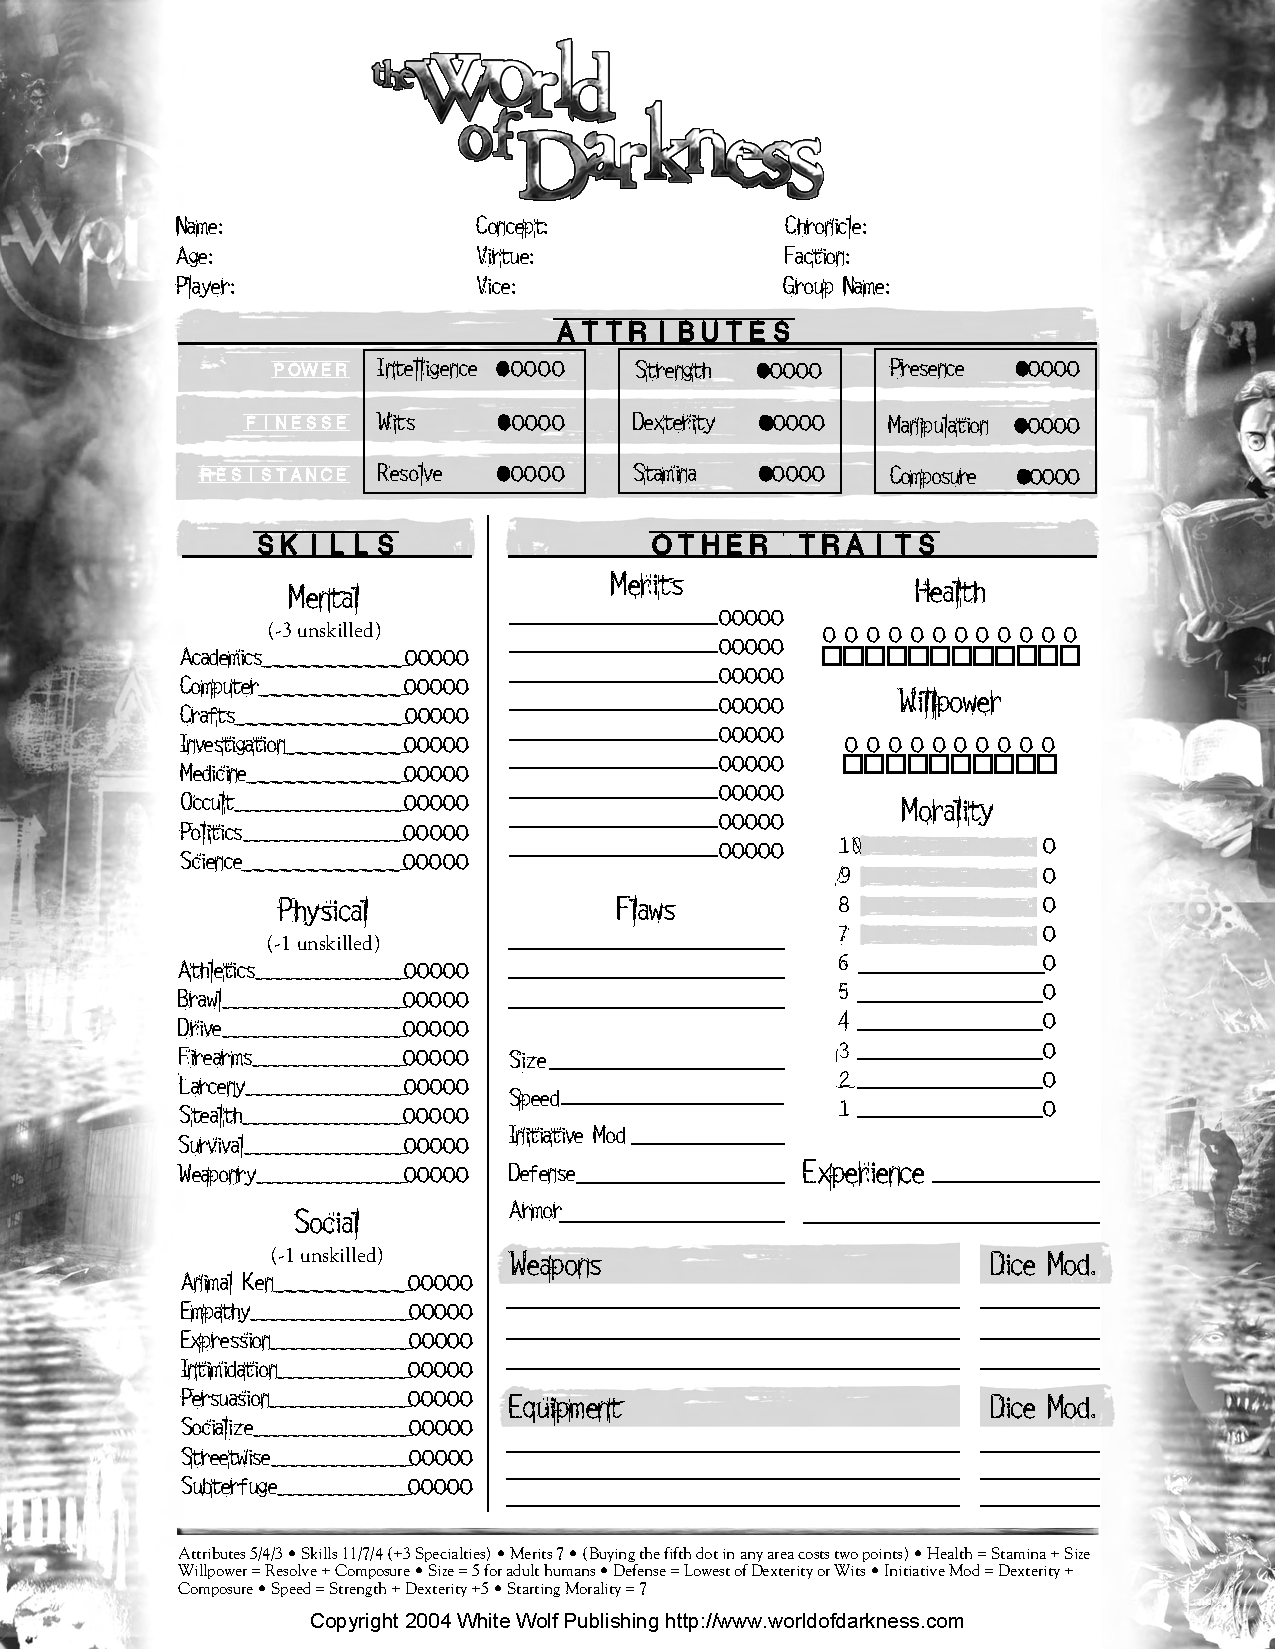
\includegraphics[scale=0.7]{tex/appendix/wodcharsheet.pdf}
%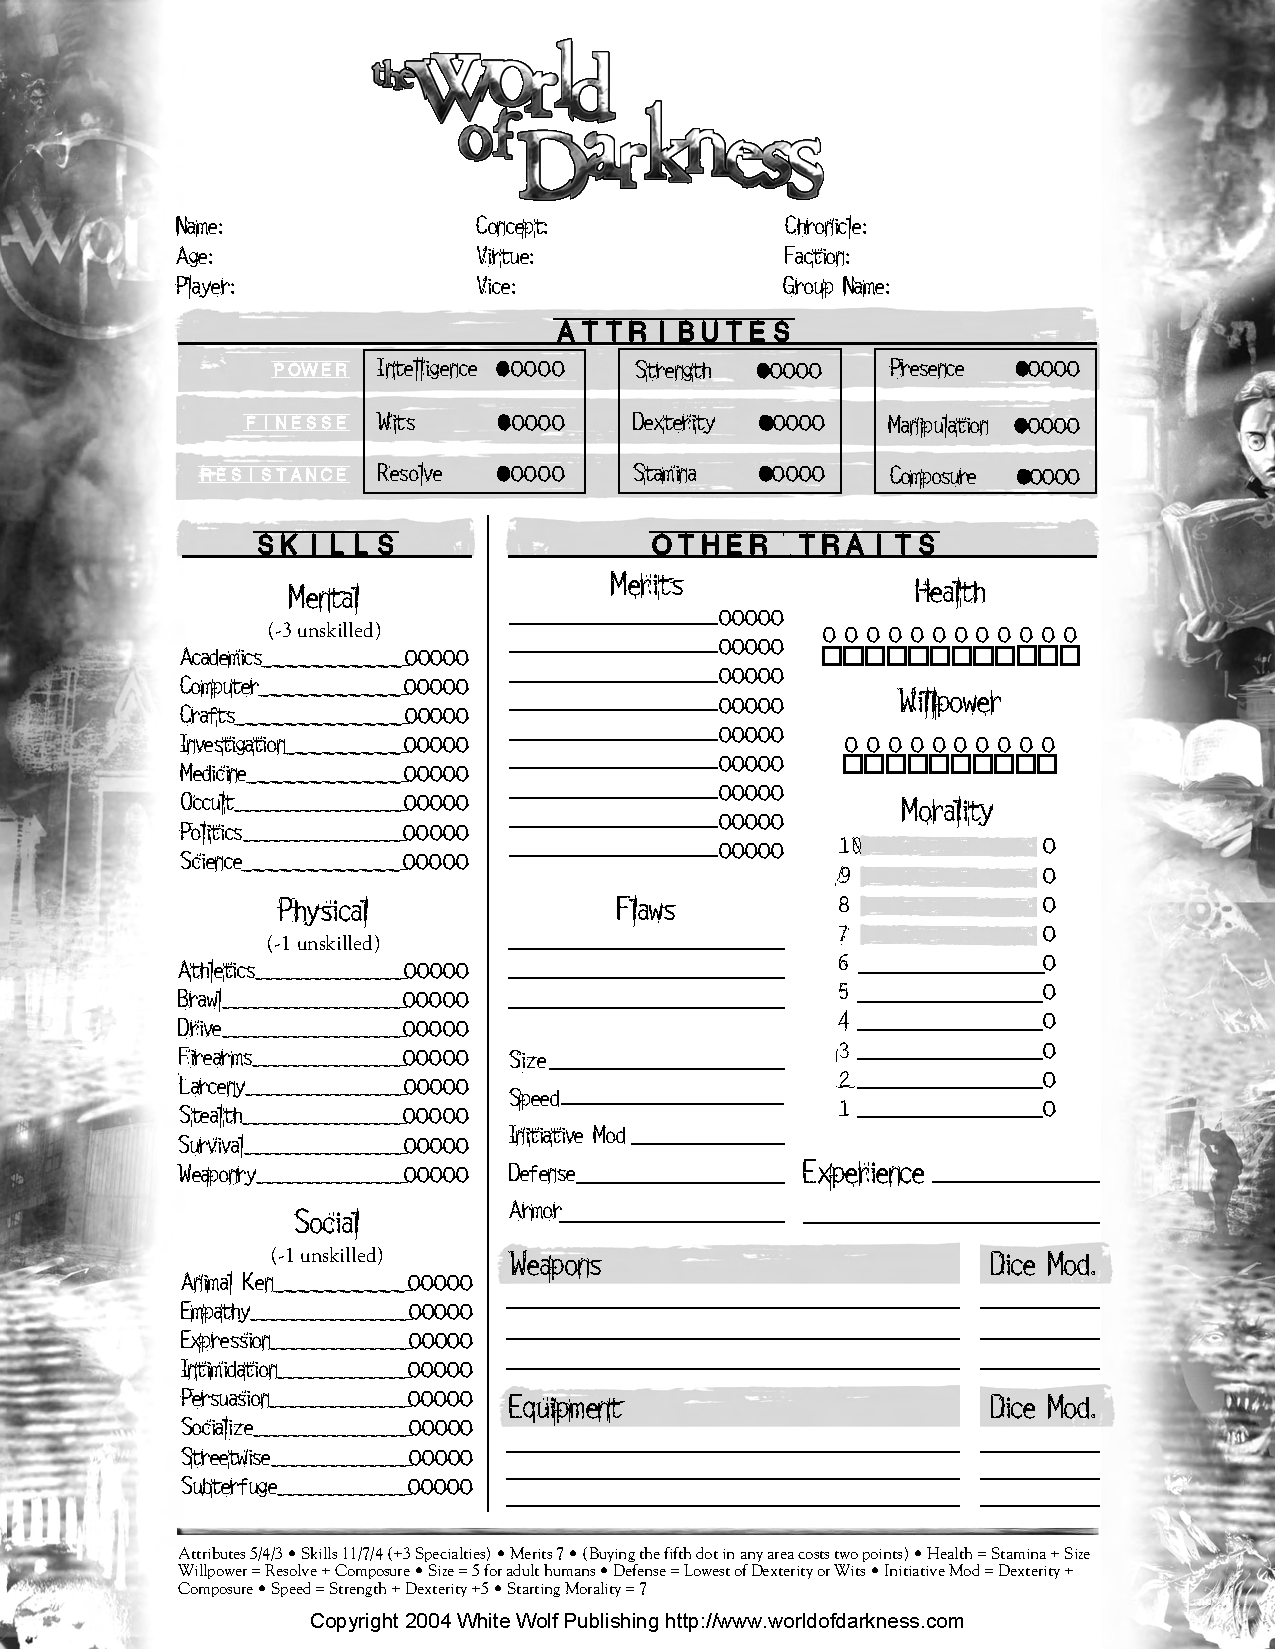
\includepdf[pages={1}, pagecommand={\label{charsheet}}]{tex/appendix/wodcharsheet.pdf}
\chapter{Character sheet}
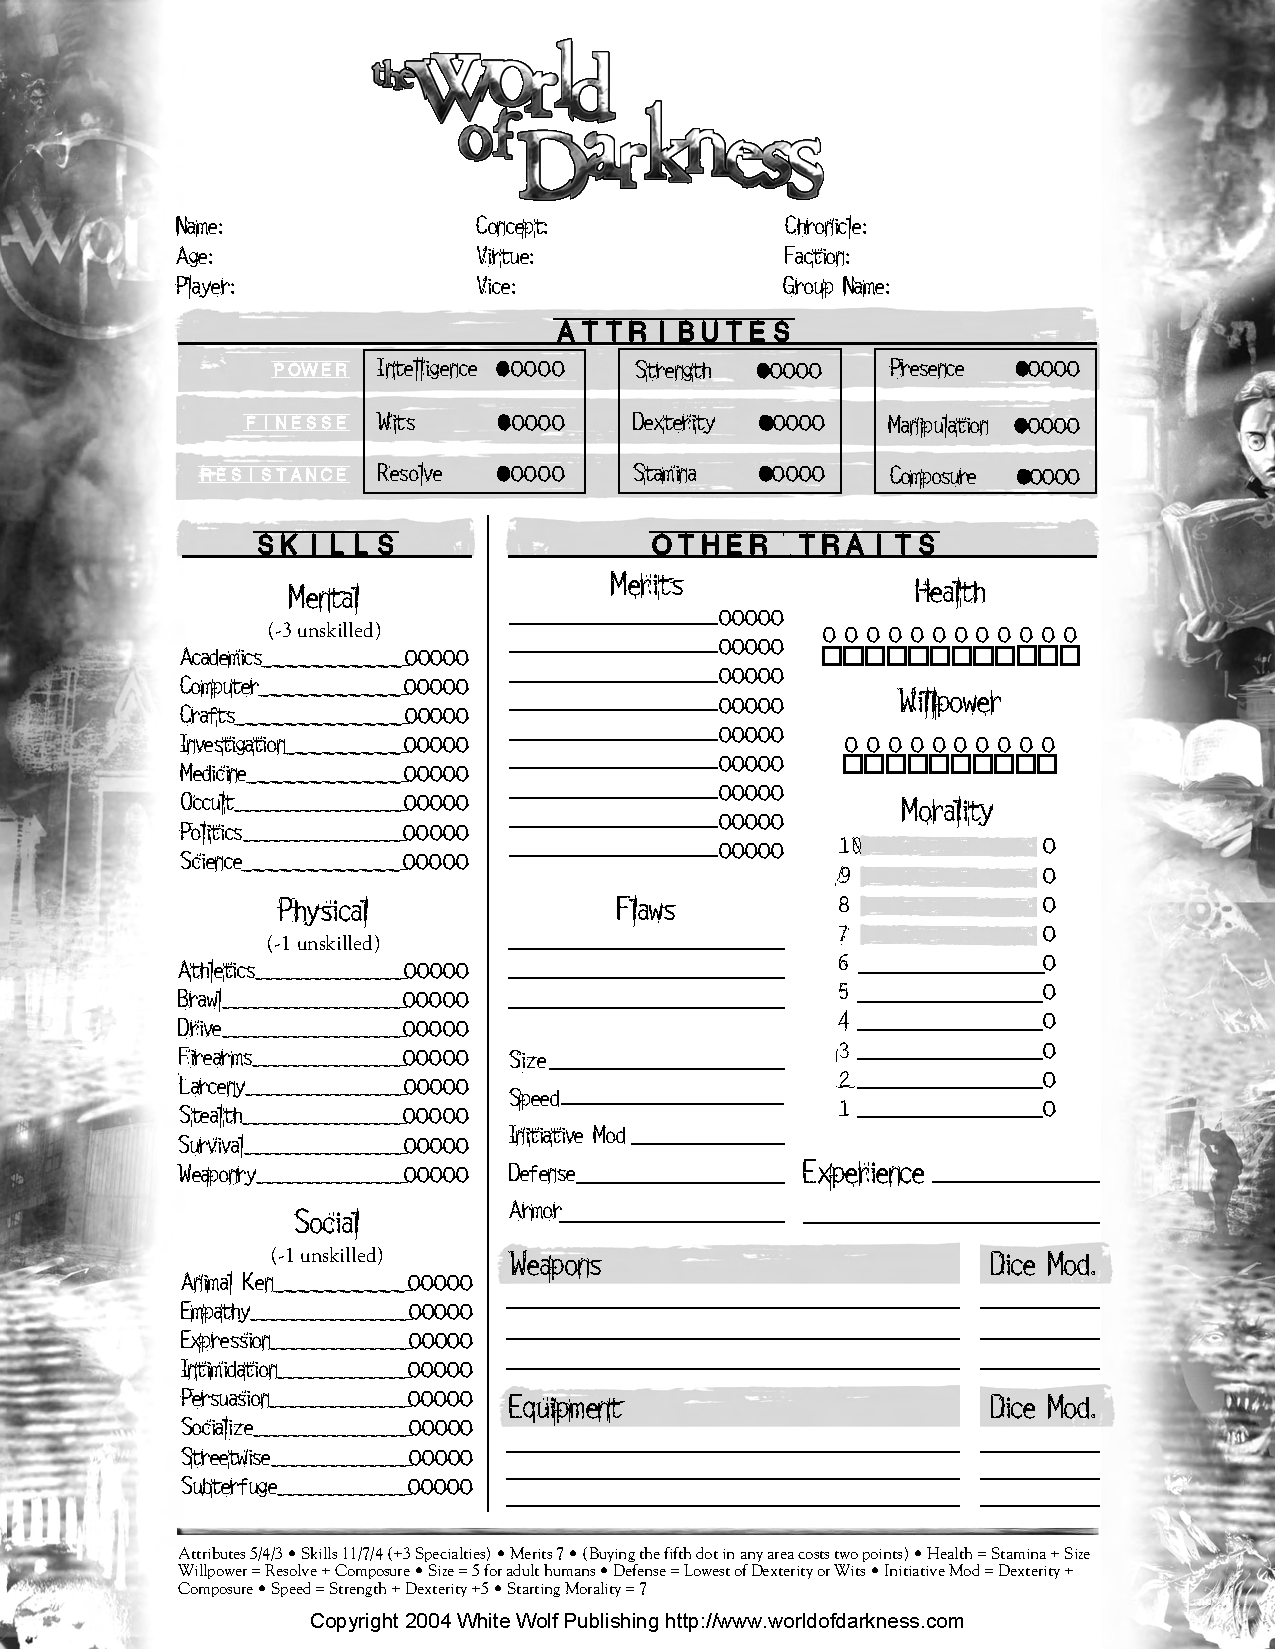
\includepdf[pages={1}, scale={0.78}, offset={0 -28}, pagecommand={\section*{Character Sheet \hfill \footnotesize{\copyright 2012 CCP hf. All rights reserved.}} \label{charsheet}}]{tex/appendix/wodcharsheet.pdf}

\end{document}
